% Konfigurationsdatei f\"ur die Pfaddefinitionen einlesen
%  se-wa-pfade.tex
%
%
%  J\"org Baumgart
%  2012-12-20
%  
%  Pfaddefinitionen (Ordnerdefinitionen) f\"ur das Einlesen von
%  -- .sty-Dateien und
%  -- Textbaustenen f\"ur die Hinweise zur Verwendung von LaTeX
%  -- jpg-Bildern
%
\newcommand{\seWaPathSty}{se-wa-styles}
\newcommand{\seWaPathText}{se-wa-textbausteine-vorlagen}
\newcommand{\seWaPathJpg}{se-wa-jpg}

%
%
% Festlegung der Sprache: 
\newcommand{\seWaSprache}{deutsch}
%\newcommand{\seWaSprache}{englisch}


%
% Einlesen der .sty-Dateien
%
%%  se-wa-input-styles-v095.tex
%
%  Joerg Baumgart 01.08.2011
%
%  Zusammenfassung und Konfiguration wichtiger Styles f\"ur die 
%  Erzeugung von Seminar-, Projekt- und Bachelorarbeiten
%
%  2012-03-12: auf Version 0.94 umgestellt
%
%
% 2012-12-13: auf Version 0.95 umgestellt
%                     Sprachoptionen englisch/deutsch zusammengef\"uhrt
%                     bchart.sty hinzugenommen
%                 
%


\documentclass[12pt,BCOR=10mm,headinclude=on,footinclude=off,bibliography=totoc]{scrreprt}
\usepackage[T1]{fontenc}
\usepackage[latin1]{inputenc}
\usepackage{ifthen}
% 2012-12-13
\ifthenelse{\equal{\seWaSprache}{deutsch}}{% Deutsche Einstellungen
\usepackage[ngerman]{babel}% 
}{% Englische Einstellungen
\usepackage[english]{babel}% 
}

\usepackage{lmodern}

\usepackage{tikz} % Graphikpaket, das zu pdfLaTeX kompatibel ist
\usepackage{xkeyval} % Definition von Kommandos mit mehreren optionalen Argumenten
\usepackage{listings} % Formatierung von Programmlistings
\usepackage{graphicx} % Einbinden von Graphiken
\usepackage{color}
\usepackage{\seWaPathSty/slashbox} % Diagonalen in Tabellenfeldern
\usepackage{framed} % Erzeugung schwarzer Linien am linken Rand zur Hervorhebung von Textteilen
\usepackage{caption} % Korrektes Setzen einer mehrzeiligen float-Unterschrift bei neu definierten float-Umgebungen
\usepackage{floatrow}
% 2012-12-13
\usepackage{\seWaPathSty/bchart} % Kommandos zur Erzeugung von Balkendiagrammen


% Es wird jeweils die sty-Datei importiert und entsprechende Konfigurationseinstellungen werden vorgenommen

\usepackage{\seWaPathSty/se-jb-scrpage2} % Formatierung der Kopf- und Fu{\ss}zeilen
\usepackage{\seWaPathSty/se-jb-footmisc}    % Fussnoten besser formatieren

\usepackage{\seWaPathSty/se-jb-glossaries-v094} % Abk\"urzungsverzeichnis, Symbolverzeichnis, Glossar
   
\usepackage{\seWaPathSty/se-jb-floatrow}    % Definition und Konfiguration von float-Umgebungen (figure, table, die neue programm-Umgebung)
% Achtung: se-jb-varioref muss nach se-jb-floatrow importiert werden; 
% andernfalls ist der counter programm f\"ur die labelformat-Anweisung noch nicht definiert   
\usepackage{\seWaPathSty/se-jb-varioref}   % Definition von Querverweisen
\usepackage{\seWaPathSty/se-jb-chngcntr}   % Kapitelweise oder globale Nummerierung von Abbildungen etc.
   
\usepackage{\seWaPathSty/se-jb-listen} % Definition neuer, besser formatierter Listen
\usepackage{\seWaPathSty/se-jb-kommandos-v095} % neue Kommandos f\"ur Seminar-, Projekt- und Bachelorarbeiten
% 2012-12-13
\ifthenelse{\equal{\seWaSprache}{englisch}}{\usepackage{\seWaPathSty/se-jb-kommandos-englisch}}{}

%  se-wa-input-styles-v095.tex
%
%  Joerg Baumgart 01.08.2011
%
%  Zusammenfassung und Konfiguration wichtiger Styles f\"ur die 
%  Erzeugung von Seminar-, Projekt- und Bachelorarbeiten
%
%  2012-03-12: auf Version 0.94 umgestellt
%
%
% 2012-12-13: auf Version 0.95 umgestellt
%                     Sprachoptionen englisch/deutsch zusammengef\"uhrt
%                     bchart.sty hinzugenommen
%                 
%


\documentclass[12pt,BCOR=10mm,headinclude=on,footinclude=off,bibliography=totoc]{scrreprt}
\usepackage[T1]{fontenc}
\usepackage[latin1]{inputenc}
\usepackage{ifthen}
% 2012-12-13
\ifthenelse{\equal{\seWaSprache}{deutsch}}{% Deutsche Einstellungen
\usepackage[ngerman]{babel}% 
}{% Englische Einstellungen
\usepackage[english]{babel}% 
}

\usepackage{lmodern}

\usepackage{tikz} % Graphikpaket, das zu pdfLaTeX kompatibel ist
\usepackage{xkeyval} % Definition von Kommandos mit mehreren optionalen Argumenten
\usepackage{listings} % Formatierung von Programmlistings
\usepackage{graphicx} % Einbinden von Graphiken
\usepackage{color}
\usepackage{\seWaPathSty/slashbox} % Diagonalen in Tabellenfeldern
\usepackage{framed} % Erzeugung schwarzer Linien am linken Rand zur Hervorhebung von Textteilen
\usepackage{caption} % Korrektes Setzen einer mehrzeiligen float-Unterschrift bei neu definierten float-Umgebungen
\usepackage{floatrow}
% 2012-12-13
\usepackage{\seWaPathSty/bchart} % Kommandos zur Erzeugung von Balkendiagrammen


% Es wird jeweils die sty-Datei importiert und entsprechende Konfigurationseinstellungen werden vorgenommen

\usepackage{\seWaPathSty/se-jb-scrpage2} % Formatierung der Kopf- und Fu{\ss}zeilen
\usepackage{\seWaPathSty/se-jb-footmisc}    % Fussnoten besser formatieren

\usepackage{\seWaPathSty/se-jb-glossaries-v094} % Abk\"urzungsverzeichnis, Symbolverzeichnis, Glossar
   
\usepackage{\seWaPathSty/se-jb-floatrow}    % Definition und Konfiguration von float-Umgebungen (figure, table, die neue programm-Umgebung)
% Achtung: se-jb-varioref muss nach se-jb-floatrow importiert werden; 
% andernfalls ist der counter programm f\"ur die labelformat-Anweisung noch nicht definiert   
\usepackage{\seWaPathSty/se-jb-varioref}   % Definition von Querverweisen
\usepackage{\seWaPathSty/se-jb-chngcntr}   % Kapitelweise oder globale Nummerierung von Abbildungen etc.
   
\usepackage{\seWaPathSty/se-jb-listen} % Definition neuer, besser formatierter Listen
\usepackage{\seWaPathSty/se-jb-kommandos-v095} % neue Kommandos f\"ur Seminar-, Projekt- und Bachelorarbeiten
% 2012-12-13
\ifthenelse{\equal{\seWaSprache}{englisch}}{\usepackage{\seWaPathSty/se-jb-kommandos-englisch}}{}


%
% Individuelle Konfiguration des Dokumentes
%
%%  Individuelle Konfiguration einer Projektarbeit/Bachelorarbeit
%
%
%
%

% 2012-10-27
%
% \"Anderung des Schrifttyps f\"ur das gesamte Dokument
%
% Das gesamte Dokument wird in einer serifenlosen Schrift gesetzt
%\renewcommand{\familydefault}{\sfdefault}
%
% Das gesamte Dokument wird in einer Serifenschrift gesetzt
% Achtung: serifenlose Schriften sind jetzt grunds\"atzlich nicht mehr nutzbar!
%
%\renewcommand{\sffamily}{\normalfont}

% 2012-12-05
%
% Verwendung des url-Pakets
% Durch den optionalen Paremeter hyphens wird eine Trennung 
% von URLs auch nach Bindestrichen erlaubt
\usepackage[hyphens]{url}


% 2012-10-27
%
%
% Literaturverzeichnis
% 
% Literaturverzeichnis gem\"ass den Vorgaben von Theisen aufbauen
\usepackage{\seWaPathSty/se-jb-jurabib-theisen} 
% Verwendung der Harvard-Zitierweise
%\usepackage{\seWaPathSty/se-jb-jurabib-harvard} 

% Weitere Optionseinstellungen f\"ur das Koma-Script
%
% Zwischen Abs\"atzen einen Abstand von 0.5 \baselineskip erzeugen
\KOMAoption{parskip}{full}
%
% Vergleiche Duden "Gliederung von Nummern, S.111" 
% DIN 5008 anschauen, wenn sie neu ver\"offentlicht wurde
\KOMAoption{numbers}{noendperiod}
%
%



%  Voreinstellungen f\"ur floats
%  Durch die verwendeten Parameter wird die Wahrscheinlichkeit deutlich kleiner, 
%  dass Gleitobjekte (z. B. Abbildungen) ans Ende des Dokumentes verschoben 
%  werden; 
%  Achtung: clearpage erzwingt die Ausgabe von Gleitobjekten
%
\renewcommand{\topfraction}{1}  % Gleitobjekte d\"urfen eine Seite zu 100% belegen 
\renewcommand{\bottomfraction}{1} % Entsprechender Wert f\"ur den unteren Teil der Seite
\renewcommand{\textfraction}{0} % Eine Seite darf auch ohne Fliesstext existieren
%%%\renewcommand{\floatpagefraction}{1} % Bedeutung unklar, daher keine Ver\"anderung des Vorgabewertes 
                                                                        % von 0.5; eventuell bringt ein \"Anderung auf 1 etwas, wenn 
                                                                         % Probleme mit floats auftreten
                                                                         
                                                                         
                                                                         
% Konfiguration von Programm-Listings
% 
% Achtung: hier gibt es nahezu beliebig viele weitere Konfigurationm\"oglichkeiten; vgl. Paketdokumentation
%
\lstset{language=Java,basicstyle=\ttfamily,keywordstyle=\color{blue},captionpos=b,aboveskip=0mm,belowskip=0mm,
          xleftmargin=0em}               
          
%
% Grundkonfiguration der Abs\"ande zwischen den Items der maximal f\"unf Verschachtelungsebenen der 
% neuen Listenumgebungen
%                                                                             
% Initialisierung der Abst\"ande zwischen den items f\"ur seList; Grundeinheit: 0.5\baselineskip; siehe se-jb-listen
\seSetlistbaselineskip{1}{0.75}{0.75}{0.75}{0.75}
% Initialisierung der Abst\"ande zwischen den items f\"ur seToplist; Grundeinheit: 0.5\baselineskip; siehe se-jb-listen
\seSettoplistbaselineskip{1}{0.75}{0.75}{0.75}{0.75}     


% Einlesen der sprachabh\"angigen Konfigurationsdatei
%
%
\ifthenelse{\equal{\seWaSprache}{deutsch}}{% deutsch
% wa-konfiguration-deutsch
%
% 2012-12-13
% 
% Diese Datei wird f\"ur die Sprachoption deutsch verwendet, d. h.  
% \newcommand{\seWaSprache}{deutsch}
%
%
% In dieser Datei k\"onnen Neudefinitionen vorgenommen werden f\"ur:
% -- Verzeichnisse
% -- Unter-/\"Uberschriften von Abbildungen, Tabellen und Listings
% -- Querverweise innerhalb des Textes

%
%  Konfiguration der verschiedenen Verzeichnisse
%
%  abstandEintrag: Wert wird mit \baselineskip multipliziert
%

%
%  Abbildungsverzeichnis
%
\seKonfigurationAbb[
%verzeichnisname=Abbildungsverzeichnis,
labeltextLinks=, % kein Text links;
%labeltextRechts=:,
labelbreite=1cm,
%labeleinzug=1cm,
%abstandEintrag=1,
%newpage=ja,
%pnumwidth=20mm,
%dotsep=1000,
%tocrmarg=4.5cm,
%abstandVerzeichnis=-1mm
]

%
% LIstingverzeichnis
%
\seKonfigurationPrg[
%verzeichnisname=Listing-Verzeichnis,
labeltextLinks=,
%labeltextRechts=:,
labelbreite=1cm,
%labeleinzug=2cm,
%abstandEintrag=1,
%newpage=ja,
%pnumwidth=20mm,
%dotsep=1000,
%tocrmarg=4.5cm,
%abstandVerzeichnis=-10mm
]

%
% Tabellenverzeichnis
%
\seKonfigurationTab[
%verzeichnisname=Liste der Tabellen,
labeltextLinks=,
%labeltextRechts=:,
labelbreite=1cm,
%labeleinzug=0.5cm,
%abstandEintrag=1,
%newpage=ja,
%pnumwidth=20mm,
%dotsep=1000,
%tocrmarg=4.5cm,
%abstandVerzeichnis=-10mm
]

%
% Abk\"urzungsverzeichnis
%
\seKonfigurationAbk[
%verzeichnisname=Liste der Abk\"urzungen,
%labelbreite=3cm,
%labeleinzug=0.5cm,
%abstandEintrag=1,
%newpage=ja,
%abstandVerzeichnis=-10mm
]

%
% Symbolverzeichnis
% 
\seKonfigurationSym[
%verzeichnisname=Liste der Symbole,
%labelbreite=4cm,
%labeleinzug=3.5cm,
%abstandEintrag=1,
%newpage=ja,
%abstandVerzeichnis=-10mm
]

%
% Glossar
%
\seKonfigurationGlo[
%verzeichnisname=Glossar,
%abstandEintrag=0,
]



% (eventuelle) Neudefinition f\"ur die Unter-/\"Uberschriften von Abbildungen, Tabellen und Listings
%
%
%\renewcommand{\seCaptionNameAbbildung}{Abb.}
%\renewcommand{\seCaptionNameTabelle}{Tab.}
%\renewcommand{\seCaptionNameProgramm}{Prg.}


% % (eventuelle) Neudefinition f\"ur Querverweise innerhalb des Textes
%
%
%
%\renewcommand{\seQuerverweisSeite}{Seite}
%\renewcommand{\seQuerverweisAbbildung}{Abb.}
%\renewcommand{\seQuerverweisTabelle}{Tab.}
%\renewcommand{\seQuerverweisProgramm}{Prg.}
%\renewcommand{\seQuerverweisGleichung}{Gl.}
%
\renewcommand{\seQuerverweisChapter}{Kapitel}
\renewcommand{\seQuerverweisSection}{Kapitel}
\renewcommand{\seQuerverweisSubsection}{Kapitel}
\renewcommand{\seQuerverweisSubsubsection}{Kapitel}
\renewcommand{\seQuerverweisParagraph}{Kapitel}


%
% Kommandos f\"ur die Konfiguration von URL-Eintr\"agen im Literaturverzeichnis
%
\renewcommand*{\biburlprefix}{\jblangle{}URL: }
\renewcommand*{\biburlsuffix}{\jbrangle{}}
\renewcommand*{\bibbudcsep}{ -- }
\AddTo\bibsgerman{\renewcommand*{\urldatecomment}{Zugriff am }}


%
}{% englisch
% wa-konfiguration-englisch
%
% 2012-12-13
% 
% Diese Datei wird f\"ur die Sprachoption englisch verwendet, d. h.  
% \newcommand{\seWaSprache}{englisch}
%
%
% In dieser Datei k\"onnen Neudefinitionen vorgenommen werden f\"ur:
% -- Verzeichnisse
% -- Unter-/\"Uberschriften von Abbildungen, Tabellen und Listings
% -- Querverweise innerhalb des Textes

%
%  Konfiguration der verschiedenen Verzeichnisse
%
%  abstandEintrag: Wert wird mit \baselineskip multipliziert
%

%
%  Abbildungsverzeichnis
%
\seKonfigurationAbb[
verzeichnisname=List of Figures,
labeltextLinks=, % kein Text links;
%labeltextRechts=:,
labelbreite=1cm,
%labeleinzug=1cm,
%abstandEintrag=1,
%newpage=ja,
%pnumwidth=20mm,
%dotsep=1000,
%tocrmarg=4.5cm,
%abstandVerzeichnis=-1mm
]

%
% LIstingverzeichnis
%
\seKonfigurationPrg[
verzeichnisname=List of Program Listings,
labeltextLinks=,
%labeltextRechts=:,
labelbreite=1cm,
%labeleinzug=2cm,
%abstandEintrag=1,
%newpage=ja,
%%pnumwidth=20mm,
%dotsep=1000,
%tocrmarg=4.5cm,
%abstandVerzeichnis=-10mm
]

%
% Tabellenverzeichnis
%
\seKonfigurationTab[
verzeichnisname=List of Tables,
labeltextLinks=,
%labeltextRechts=:,
labelbreite=1cm,
%labeleinzug=0.5cm,
%abstandEintrag=1,
%newpage=ja,
%pnumwidth=20mm,
%dotsep=1000,
%tocrmarg=4.5cm,
%abstandVerzeichnis=-10mm
]

%
% Abk\"urzungsverzeichnis
%
\seKonfigurationAbk[
verzeichnisname=List of Abbreviations,
%labelbreite=3cm,
%labeleinzug=0.5cm,
%abstandEintrag=1,
%newpage=ja,
%abstandVerzeichnis=-10mm
]

%
% Symbolverzeichnis
% 
\seKonfigurationSym[
verzeichnisname=List of Symbols,
%labelbreite=4cm,
%labeleinzug=3.5cm,
%abstandEintrag=1,
%newpage=ja,
%abstandVerzeichnis=-10mm
]

%
% Glossar
%
\seKonfigurationGlo[
verzeichnisname=Glossary,
%abstandEintrag=0,
]



% (eventuelle) Neudefinition f\"ur die Unter-/\"Uberschriften von Abbildungen, Tabellen und Listings
%
%
\renewcommand{\seCaptionNameAbbildung}{Figure}
\renewcommand{\seCaptionNameTabelle}{Table}
\renewcommand{\seCaptionNameProgramm}{Listing}


% % (eventuelle) Neudefinition f\"ur Querverweise innerhalb des Textes
%
%
%
\renewcommand{\seQuerverweisSeite}{page}
\renewcommand{\seQuerverweisAbbildung}{figure}
\renewcommand{\seQuerverweisTabelle}{table}
\renewcommand{\seQuerverweisProgramm}{listing}
\renewcommand{\seQuerverweisGleichung}{equation}
%
\renewcommand{\seQuerverweisChapter}{chapter}
\renewcommand{\seQuerverweisSection}{chapter}
\renewcommand{\seQuerverweisSubsection}{chapter}
\renewcommand{\seQuerverweisSubsubsection}{chapter}
\renewcommand{\seQuerverweisParagraph}{chapter}


%
% Kommandos f\"ur die Konfiguration von URL-Eintr\"agen im Literaturverzeichnis
%
\renewcommand*{\biburlprefix}{\jblangle{}URL: }
\renewcommand*{\biburlsuffix}{\jbrangle{}}
\renewcommand*{\bibbudcsep}{ -- }
\AddTo\bibsenglish{\renewcommand*{\urldatecomment}{visited on }}


}

% Kommandos, die direkt nach \begin{document} ausgef\"uhrt werden m\"ussen
%
%
%
\AtBeginDocument{%
\renewcommand{\listfigurename}{\seAbbildungenVerzeichnisname}
\renewcommand{\listtablename}{\seTabellenVerzeichnisname}
\renewcommand{\figurename}{\seCaptionNameAbbildung}
\renewcommand{\tablename}{\seCaptionNameTabelle}
\pagenumbering{roman}
}
                                                              
                                                                         
%  Individuelle Konfiguration einer Projektarbeit/Bachelorarbeit
%
%
%
%

% 2012-10-27
%
% \"Anderung des Schrifttyps f\"ur das gesamte Dokument
%
% Das gesamte Dokument wird in einer serifenlosen Schrift gesetzt
%\renewcommand{\familydefault}{\sfdefault}
%
% Das gesamte Dokument wird in einer Serifenschrift gesetzt
% Achtung: serifenlose Schriften sind jetzt grunds\"atzlich nicht mehr nutzbar!
%
%\renewcommand{\sffamily}{\normalfont}

% 2012-12-05
%
% Verwendung des url-Pakets
% Durch den optionalen Paremeter hyphens wird eine Trennung 
% von URLs auch nach Bindestrichen erlaubt
\usepackage[hyphens]{url}


% 2012-10-27
%
%
% Literaturverzeichnis
% 
% Literaturverzeichnis gem\"ass den Vorgaben von Theisen aufbauen
\usepackage{\seWaPathSty/se-jb-jurabib-theisen} 
% Verwendung der Harvard-Zitierweise
%\usepackage{\seWaPathSty/se-jb-jurabib-harvard} 

% Weitere Optionseinstellungen f\"ur das Koma-Script
%
% Zwischen Abs\"atzen einen Abstand von 0.5 \baselineskip erzeugen
\KOMAoption{parskip}{full}
%
% Vergleiche Duden "Gliederung von Nummern, S.111" 
% DIN 5008 anschauen, wenn sie neu ver\"offentlicht wurde
\KOMAoption{numbers}{noendperiod}
%
%



%  Voreinstellungen f\"ur floats
%  Durch die verwendeten Parameter wird die Wahrscheinlichkeit deutlich kleiner, 
%  dass Gleitobjekte (z. B. Abbildungen) ans Ende des Dokumentes verschoben 
%  werden; 
%  Achtung: clearpage erzwingt die Ausgabe von Gleitobjekten
%
\renewcommand{\topfraction}{1}  % Gleitobjekte d\"urfen eine Seite zu 100% belegen 
\renewcommand{\bottomfraction}{1} % Entsprechender Wert f\"ur den unteren Teil der Seite
\renewcommand{\textfraction}{0} % Eine Seite darf auch ohne Fliesstext existieren
%%%\renewcommand{\floatpagefraction}{1} % Bedeutung unklar, daher keine Ver\"anderung des Vorgabewertes 
                                                                        % von 0.5; eventuell bringt ein \"Anderung auf 1 etwas, wenn 
                                                                         % Probleme mit floats auftreten
                                                                         
                                                                         
                                                                         
% Konfiguration von Programm-Listings
% 
% Achtung: hier gibt es nahezu beliebig viele weitere Konfigurationm\"oglichkeiten; vgl. Paketdokumentation
%
\lstset{language=Java,basicstyle=\ttfamily,keywordstyle=\color{blue},captionpos=b,aboveskip=0mm,belowskip=0mm,
          xleftmargin=0em}               
          
%
% Grundkonfiguration der Abs\"ande zwischen den Items der maximal f\"unf Verschachtelungsebenen der 
% neuen Listenumgebungen
%                                                                             
% Initialisierung der Abst\"ande zwischen den items f\"ur seList; Grundeinheit: 0.5\baselineskip; siehe se-jb-listen
\seSetlistbaselineskip{1}{0.75}{0.75}{0.75}{0.75}
% Initialisierung der Abst\"ande zwischen den items f\"ur seToplist; Grundeinheit: 0.5\baselineskip; siehe se-jb-listen
\seSettoplistbaselineskip{1}{0.75}{0.75}{0.75}{0.75}     


% Einlesen der sprachabh\"angigen Konfigurationsdatei
%
%
\ifthenelse{\equal{\seWaSprache}{deutsch}}{% deutsch
% wa-konfiguration-deutsch
%
% 2012-12-13
% 
% Diese Datei wird f\"ur die Sprachoption deutsch verwendet, d. h.  
% \newcommand{\seWaSprache}{deutsch}
%
%
% In dieser Datei k\"onnen Neudefinitionen vorgenommen werden f\"ur:
% -- Verzeichnisse
% -- Unter-/\"Uberschriften von Abbildungen, Tabellen und Listings
% -- Querverweise innerhalb des Textes

%
%  Konfiguration der verschiedenen Verzeichnisse
%
%  abstandEintrag: Wert wird mit \baselineskip multipliziert
%

%
%  Abbildungsverzeichnis
%
\seKonfigurationAbb[
%verzeichnisname=Abbildungsverzeichnis,
labeltextLinks=, % kein Text links;
%labeltextRechts=:,
labelbreite=1cm,
%labeleinzug=1cm,
%abstandEintrag=1,
%newpage=ja,
%pnumwidth=20mm,
%dotsep=1000,
%tocrmarg=4.5cm,
%abstandVerzeichnis=-1mm
]

%
% LIstingverzeichnis
%
\seKonfigurationPrg[
%verzeichnisname=Listing-Verzeichnis,
labeltextLinks=,
%labeltextRechts=:,
labelbreite=1cm,
%labeleinzug=2cm,
%abstandEintrag=1,
%newpage=ja,
%pnumwidth=20mm,
%dotsep=1000,
%tocrmarg=4.5cm,
%abstandVerzeichnis=-10mm
]

%
% Tabellenverzeichnis
%
\seKonfigurationTab[
%verzeichnisname=Liste der Tabellen,
labeltextLinks=,
%labeltextRechts=:,
labelbreite=1cm,
%labeleinzug=0.5cm,
%abstandEintrag=1,
%newpage=ja,
%pnumwidth=20mm,
%dotsep=1000,
%tocrmarg=4.5cm,
%abstandVerzeichnis=-10mm
]

%
% Abk\"urzungsverzeichnis
%
\seKonfigurationAbk[
%verzeichnisname=Liste der Abk\"urzungen,
%labelbreite=3cm,
%labeleinzug=0.5cm,
%abstandEintrag=1,
%newpage=ja,
%abstandVerzeichnis=-10mm
]

%
% Symbolverzeichnis
% 
\seKonfigurationSym[
%verzeichnisname=Liste der Symbole,
%labelbreite=4cm,
%labeleinzug=3.5cm,
%abstandEintrag=1,
%newpage=ja,
%abstandVerzeichnis=-10mm
]

%
% Glossar
%
\seKonfigurationGlo[
%verzeichnisname=Glossar,
%abstandEintrag=0,
]



% (eventuelle) Neudefinition f\"ur die Unter-/\"Uberschriften von Abbildungen, Tabellen und Listings
%
%
%\renewcommand{\seCaptionNameAbbildung}{Abb.}
%\renewcommand{\seCaptionNameTabelle}{Tab.}
%\renewcommand{\seCaptionNameProgramm}{Prg.}


% % (eventuelle) Neudefinition f\"ur Querverweise innerhalb des Textes
%
%
%
%\renewcommand{\seQuerverweisSeite}{Seite}
%\renewcommand{\seQuerverweisAbbildung}{Abb.}
%\renewcommand{\seQuerverweisTabelle}{Tab.}
%\renewcommand{\seQuerverweisProgramm}{Prg.}
%\renewcommand{\seQuerverweisGleichung}{Gl.}
%
\renewcommand{\seQuerverweisChapter}{Kapitel}
\renewcommand{\seQuerverweisSection}{Kapitel}
\renewcommand{\seQuerverweisSubsection}{Kapitel}
\renewcommand{\seQuerverweisSubsubsection}{Kapitel}
\renewcommand{\seQuerverweisParagraph}{Kapitel}


%
% Kommandos f\"ur die Konfiguration von URL-Eintr\"agen im Literaturverzeichnis
%
\renewcommand*{\biburlprefix}{\jblangle{}URL: }
\renewcommand*{\biburlsuffix}{\jbrangle{}}
\renewcommand*{\bibbudcsep}{ -- }
\AddTo\bibsgerman{\renewcommand*{\urldatecomment}{Zugriff am }}


%
}{% englisch
% wa-konfiguration-englisch
%
% 2012-12-13
% 
% Diese Datei wird f\"ur die Sprachoption englisch verwendet, d. h.  
% \newcommand{\seWaSprache}{englisch}
%
%
% In dieser Datei k\"onnen Neudefinitionen vorgenommen werden f\"ur:
% -- Verzeichnisse
% -- Unter-/\"Uberschriften von Abbildungen, Tabellen und Listings
% -- Querverweise innerhalb des Textes

%
%  Konfiguration der verschiedenen Verzeichnisse
%
%  abstandEintrag: Wert wird mit \baselineskip multipliziert
%

%
%  Abbildungsverzeichnis
%
\seKonfigurationAbb[
verzeichnisname=List of Figures,
labeltextLinks=, % kein Text links;
%labeltextRechts=:,
labelbreite=1cm,
%labeleinzug=1cm,
%abstandEintrag=1,
%newpage=ja,
%pnumwidth=20mm,
%dotsep=1000,
%tocrmarg=4.5cm,
%abstandVerzeichnis=-1mm
]

%
% LIstingverzeichnis
%
\seKonfigurationPrg[
verzeichnisname=List of Program Listings,
labeltextLinks=,
%labeltextRechts=:,
labelbreite=1cm,
%labeleinzug=2cm,
%abstandEintrag=1,
%newpage=ja,
%%pnumwidth=20mm,
%dotsep=1000,
%tocrmarg=4.5cm,
%abstandVerzeichnis=-10mm
]

%
% Tabellenverzeichnis
%
\seKonfigurationTab[
verzeichnisname=List of Tables,
labeltextLinks=,
%labeltextRechts=:,
labelbreite=1cm,
%labeleinzug=0.5cm,
%abstandEintrag=1,
%newpage=ja,
%pnumwidth=20mm,
%dotsep=1000,
%tocrmarg=4.5cm,
%abstandVerzeichnis=-10mm
]

%
% Abk\"urzungsverzeichnis
%
\seKonfigurationAbk[
verzeichnisname=List of Abbreviations,
%labelbreite=3cm,
%labeleinzug=0.5cm,
%abstandEintrag=1,
%newpage=ja,
%abstandVerzeichnis=-10mm
]

%
% Symbolverzeichnis
% 
\seKonfigurationSym[
verzeichnisname=List of Symbols,
%labelbreite=4cm,
%labeleinzug=3.5cm,
%abstandEintrag=1,
%newpage=ja,
%abstandVerzeichnis=-10mm
]

%
% Glossar
%
\seKonfigurationGlo[
verzeichnisname=Glossary,
%abstandEintrag=0,
]



% (eventuelle) Neudefinition f\"ur die Unter-/\"Uberschriften von Abbildungen, Tabellen und Listings
%
%
\renewcommand{\seCaptionNameAbbildung}{Figure}
\renewcommand{\seCaptionNameTabelle}{Table}
\renewcommand{\seCaptionNameProgramm}{Listing}


% % (eventuelle) Neudefinition f\"ur Querverweise innerhalb des Textes
%
%
%
\renewcommand{\seQuerverweisSeite}{page}
\renewcommand{\seQuerverweisAbbildung}{figure}
\renewcommand{\seQuerverweisTabelle}{table}
\renewcommand{\seQuerverweisProgramm}{listing}
\renewcommand{\seQuerverweisGleichung}{equation}
%
\renewcommand{\seQuerverweisChapter}{chapter}
\renewcommand{\seQuerverweisSection}{chapter}
\renewcommand{\seQuerverweisSubsection}{chapter}
\renewcommand{\seQuerverweisSubsubsection}{chapter}
\renewcommand{\seQuerverweisParagraph}{chapter}


%
% Kommandos f\"ur die Konfiguration von URL-Eintr\"agen im Literaturverzeichnis
%
\renewcommand*{\biburlprefix}{\jblangle{}URL: }
\renewcommand*{\biburlsuffix}{\jbrangle{}}
\renewcommand*{\bibbudcsep}{ -- }
\AddTo\bibsenglish{\renewcommand*{\urldatecomment}{visited on }}


}

% Kommandos, die direkt nach \begin{document} ausgef\"uhrt werden m\"ussen
%
%
%
\AtBeginDocument{%
\renewcommand{\listfigurename}{\seAbbildungenVerzeichnisname}
\renewcommand{\listtablename}{\seTabellenVerzeichnisname}
\renewcommand{\figurename}{\seCaptionNameAbbildung}
\renewcommand{\tablename}{\seCaptionNameTabelle}
\pagenumbering{roman}
}
                                                              
                                                                         

%
% Definition von Abk\"urzungen, Symbolen und eventuell Glossareintr\"agen
%
%% 2012-03-22 Verwendung des optionalen Parameters f\"ur die Pluralform einer Abk\"urzung
%
% 2012-02-06 Umstellung auf die neuen Kommandos
%
%
%
%  J\"org Baumgart
%  Definition einiger Abk\"urzungen
%  


% Definition von Abk\"urzungen
%
% 1. Parameter: Schluessel (key) der Abkuerzung
% 2. Parameter: Abkuerzung
% 3. Parameter: Vollform
% 4. Parameter: Vollform im Plural (optional; falls nicht definiert, wird der Wert des dritten Parameters verwendet)
%
\seNewAcronymEntry{dm}{DM}{Diagonalmatrix}{Diagonalmatrizen}

\seNewAcronymEntry{dhbw}{DHBW}{Duale Hochschule Baden-W\"urttemberg}{}{}

\seNewAcronymEntry{usb}{USB}{Universal Serial Bus}{}

\seNewAcronymEntry{ctan}{CTAN}{Comprehensive \TeX{} Archive Network}{}


% 2012-03-24
% \"Uber den optionalen Parameter in eckigen Klammern wird die Pluralform f\"ur das erste 
% Auftreten der Abk\"urzung definiert

\seNewAcronymEntry[URLs]{url}{URL}{Uniform Resource Locator}%
{Uniform Resource Locators}


% Definition von Symbolen
%
% 1. Parameter: Schluessel (key) des Symbols
% 2. Parameter: Symbol
% 3. Parameter: Text, der die Sortierreihenfolge festlegt (optional; falls nicht definiert, wird der Wert des zweiten 
%                        Parameters verwendet)
% 4. Parameter: Beschreibung des Symbols
%

\seNewSymbolEntry{ND}{ND}{a}{Nutzungsdauer einer Maschine}

\seNewSymbolEntry{pi}{$\pi$}{b}{Die Kreiszahl}




% Definition von Glossareintraegen
%
% 1. Parameter: Schluessel (key) des Glossareintrags
% 2. Parameter: Begriff, der im Glossar definiert wird
% 3. Parameter: Pluralform des Begriffes (optional; falls nicht definiert, wird der Wert des zweiten Parameters verwendet)
%                        Achtung: Pluralform gilt nur fuer das erste Auftreten des Begriffes im Text
% 4. Parameter: Beschreibung des Glossareintrags
%
%
%

\seNewGlossaryEntry{glos:AD}{Active Directory}{Active Directories}
{Active Directory ist in einem Windows 2000/Windows
Server 2003-Netzwerk der Verzeichnisdienst, der die zentrale
Organisation und Verwaltung aller Netzwerkressourcen erlaubt. Es
erm\"oglicht den Benutzern \"uber eine einzige zentrale Anmeldung den
Zugriff auf alle Ressourcen und den Administratoren die zentral
organisierte Verwaltung, transparent von der Netzwerktopologie und
den eingesetzten Netzwerkprotokollen. Das daf\"ur ben\"otigte
Betriebssystem ist entweder Windows 2000 Server oder
Windows Server 2003, welches auf dem zentralen
Dom\"anencontroller installiert wird. Dieser h\"alt alle Daten des
Active Directory vor, wie z.\,B. Benutzernamen und
Kennw\"orter.\protect\seFootcite{Vgl.}{S. 200}{Dud09}}


\seNewGlossaryEntry{glos:bs}{Betriebssystem}{Betriebssysteme}{Die Begriffsdefinition sollten Sie eigentlich kennen!}


% Definition von Glossareintraegen, die gleichzeitig im Abk�rzungsverzeichnis auftreten
%
% 1. Parameter: Schluessel (key) des Glossareintrags
% 2. Parameter: Abk\"urzung
% 3. Parameter: Vollform
% 4. Parameter: Vollform im Plural (optional; falls nicht definiert, wird der Wert des dritten Parameters verwendet)
% 5. Parameter: Beschreibung des Glossareintrags

\seNewAcronymGlossaryEntry{glos:ma}{MA}{Mobile Applikation}{Mobile Applikationen}
{Eine Applikation, die auf einem mobilen Endger\"at ausgef\"uhrt wird.}

% 2012-03-24
% \"Uber den optionalen Parameter in eckigen Klammern wird die Pluralform f\"ur die Abk\"urzung definiert

\seNewAcronymGlossaryEntry[TAen]{glos:ta}{TA}{Transaktion}%
{Transaktionen}%
{Was eine Transaktion ist, sollten Sie ebenfalls bereits wissen!}





% Alternative Definition von Abk\"urzungen; diese sollten nicht verwendet werden!!!
%
%\newacronym{dhbw}{DHBW}{Duale Hochschule Baden-W\"urttemberg}
%\newacronym{usb}{USB}{Universal Serial Bus}


% Alternative Definition von Symbolen
%
% Achtung: ohne sort wird nach Name sortiert
%\newglossaryentry{pi}{
%name=$\pi$,
%description={Die Kreiszahl},
%type=symbolslist,
%sort=b
%}
%
%\newglossaryentry{ND}{
%name=$\mbox{\textsl{ND}}$,
%description={Nutzungsdauer einer Maschine},
%type=symbolslist,%
%sort=a
%}



% Alternative Definition von Glossareintr\"agen
%
%\newglossaryentry{glos:AD}{
%first=Active Directory\textsuperscript{GL},
%name=Active Directory,
%description={Active Directory ist in einem Windows 2000/Windows
%Server 2003-Netzwerk der Verzeichnisdienst, der die zentrale
%Organisation und Verwaltung aller Netzwerkressourcen erlaubt. Es
%erm\"oglicht den Benutzern \"uber eine einzige zentrale Anmeldung den
%Zugriff auf alle Ressourcen und den Administratoren die zentral
%organisierte Verwaltung, transparent von der Netzwerktopologie und
%den eingesetzten Netzwerkprotokollen. Das daf\"ur ben\"otigte
%Betriebssystem ist entweder Windows 2000 Server oder
%Windows Server 2003, welches auf dem zentralen
%Dom\"anencontroller installiert wird. Dieser h\"alt alle Daten des
%Active Directory vor, wie z.\,B. Benutzernamen und
%Kennw\"orter.\protect\seFootcite{Vgl.}{S. 200}{Dud09}}
%}














 
% 2012-03-22 Verwendung des optionalen Parameters f\"ur die Pluralform einer Abk\"urzung
%
% 2012-02-06 Umstellung auf die neuen Kommandos
%
%
%
%  J\"org Baumgart
%  Definition einiger Abk\"urzungen
%  


% Definition von Abk\"urzungen
%
% 1. Parameter: Schluessel (key) der Abkuerzung
% 2. Parameter: Abkuerzung
% 3. Parameter: Vollform
% 4. Parameter: Vollform im Plural (optional; falls nicht definiert, wird der Wert des dritten Parameters verwendet)
%
\seNewAcronymEntry{dm}{DM}{Diagonalmatrix}{Diagonalmatrizen}

\seNewAcronymEntry{dhbw}{DHBW}{Duale Hochschule Baden-W\"urttemberg}{}{}

\seNewAcronymEntry{usb}{USB}{Universal Serial Bus}{}

\seNewAcronymEntry{ctan}{CTAN}{Comprehensive \TeX{} Archive Network}{}


% 2012-03-24
% \"Uber den optionalen Parameter in eckigen Klammern wird die Pluralform f\"ur das erste 
% Auftreten der Abk\"urzung definiert

\seNewAcronymEntry[URLs]{url}{URL}{Uniform Resource Locator}%
{Uniform Resource Locators}


% Definition von Symbolen
%
% 1. Parameter: Schluessel (key) des Symbols
% 2. Parameter: Symbol
% 3. Parameter: Text, der die Sortierreihenfolge festlegt (optional; falls nicht definiert, wird der Wert des zweiten 
%                        Parameters verwendet)
% 4. Parameter: Beschreibung des Symbols
%

\seNewSymbolEntry{ND}{ND}{a}{Nutzungsdauer einer Maschine}

\seNewSymbolEntry{pi}{$\pi$}{b}{Die Kreiszahl}




% Definition von Glossareintraegen
%
% 1. Parameter: Schluessel (key) des Glossareintrags
% 2. Parameter: Begriff, der im Glossar definiert wird
% 3. Parameter: Pluralform des Begriffes (optional; falls nicht definiert, wird der Wert des zweiten Parameters verwendet)
%                        Achtung: Pluralform gilt nur fuer das erste Auftreten des Begriffes im Text
% 4. Parameter: Beschreibung des Glossareintrags
%
%
%

\seNewGlossaryEntry{glos:AD}{Active Directory}{Active Directories}
{Active Directory ist in einem Windows 2000/Windows
Server 2003-Netzwerk der Verzeichnisdienst, der die zentrale
Organisation und Verwaltung aller Netzwerkressourcen erlaubt. Es
erm\"oglicht den Benutzern \"uber eine einzige zentrale Anmeldung den
Zugriff auf alle Ressourcen und den Administratoren die zentral
organisierte Verwaltung, transparent von der Netzwerktopologie und
den eingesetzten Netzwerkprotokollen. Das daf\"ur ben\"otigte
Betriebssystem ist entweder Windows 2000 Server oder
Windows Server 2003, welches auf dem zentralen
Dom\"anencontroller installiert wird. Dieser h\"alt alle Daten des
Active Directory vor, wie z.\,B. Benutzernamen und
Kennw\"orter.\protect\seFootcite{Vgl.}{S. 200}{Dud09}}


\seNewGlossaryEntry{glos:bs}{Betriebssystem}{Betriebssysteme}{Die Begriffsdefinition sollten Sie eigentlich kennen!}


% Definition von Glossareintraegen, die gleichzeitig im Abk�rzungsverzeichnis auftreten
%
% 1. Parameter: Schluessel (key) des Glossareintrags
% 2. Parameter: Abk\"urzung
% 3. Parameter: Vollform
% 4. Parameter: Vollform im Plural (optional; falls nicht definiert, wird der Wert des dritten Parameters verwendet)
% 5. Parameter: Beschreibung des Glossareintrags

\seNewAcronymGlossaryEntry{glos:ma}{MA}{Mobile Applikation}{Mobile Applikationen}
{Eine Applikation, die auf einem mobilen Endger\"at ausgef\"uhrt wird.}

% 2012-03-24
% \"Uber den optionalen Parameter in eckigen Klammern wird die Pluralform f\"ur die Abk\"urzung definiert

\seNewAcronymGlossaryEntry[TAen]{glos:ta}{TA}{Transaktion}%
{Transaktionen}%
{Was eine Transaktion ist, sollten Sie ebenfalls bereits wissen!}





% Alternative Definition von Abk\"urzungen; diese sollten nicht verwendet werden!!!
%
%\newacronym{dhbw}{DHBW}{Duale Hochschule Baden-W\"urttemberg}
%\newacronym{usb}{USB}{Universal Serial Bus}


% Alternative Definition von Symbolen
%
% Achtung: ohne sort wird nach Name sortiert
%\newglossaryentry{pi}{
%name=$\pi$,
%description={Die Kreiszahl},
%type=symbolslist,
%sort=b
%}
%
%\newglossaryentry{ND}{
%name=$\mbox{\textsl{ND}}$,
%description={Nutzungsdauer einer Maschine},
%type=symbolslist,%
%sort=a
%}



% Alternative Definition von Glossareintr\"agen
%
%\newglossaryentry{glos:AD}{
%first=Active Directory\textsuperscript{GL},
%name=Active Directory,
%description={Active Directory ist in einem Windows 2000/Windows
%Server 2003-Netzwerk der Verzeichnisdienst, der die zentrale
%Organisation und Verwaltung aller Netzwerkressourcen erlaubt. Es
%erm\"oglicht den Benutzern \"uber eine einzige zentrale Anmeldung den
%Zugriff auf alle Ressourcen und den Administratoren die zentral
%organisierte Verwaltung, transparent von der Netzwerktopologie und
%den eingesetzten Netzwerkprotokollen. Das daf\"ur ben\"otigte
%Betriebssystem ist entweder Windows 2000 Server oder
%Windows Server 2003, welches auf dem zentralen
%Dom\"anencontroller installiert wird. Dieser h\"alt alle Daten des
%Active Directory vor, wie z.\,B. Benutzernamen und
%Kennw\"orter.\protect\seFootcite{Vgl.}{S. 200}{Dud09}}
%}
















\seIstSeminararbeit{}

\newcommand{\version}{0.953}

% 
% Diese Redefinition ist nur f\"ur den Anhang der  
% Vorlage (Hinweise zur Installation und \"Ubersetzung)
% notwendig; f\"ur Ihre Seminar-/Projekt-/Bachelorarbeit spielt sie keine Rolle
%
\renewcommand{\seVorlage}{\jobname}

% Verwendung kleinerer Schriftgroessen f�r die Ueberschriften; sinnvoll bei kurzen Texten.
%
%
\KOMAoption{headings}{small}

% Fuer einen Kapitelanfang wird kein zusaetzlicher vertikaler Abstand erzeugt
%
%
\seNoChapterSkip[-12.25mm]{}

\begin{document}		
% Erzeugung des Titelblatts
%
%
%
\seTitelblattSeminararbeit[
%hilfslinien=ja,
%dhbwlogoSkalierung=0.5,
%dhbwlogoDeltaX=2.4,
%dhbwlogoDeltaY=-10,
studiengang=\seWirtschaftsinformatik,
studienrichtung=\seSoftwareEngineering,
thema=Fallstudie,
verfasser={J�rn H�bner , Patrick Knerr, Marco Riege, Matthias Liedtke, Oliver
Frendo},
%verfasserin= Melanie Musterfrau,
kurs=WWI\,12\,SE\,B,
firma=SAP,
% Da im Text ein Komma enthalten ist, muss der Text eingeklammert werden
%studiengangsleiterin=,
studiengangsleiter=Prof. Dr. Herr Holey,
modul=Umsetzung von Methoden der Wirtschaftsinformatik,
lehrveranstaltung=Fallstudie,
%dozentin=,
dozent=Gregor Tielsch
]


% Erzeugung der englischen Kurzfassung (Abstract); Verfasser, Firma und Thema werden automatisch \"ubernommen
%
% Der optionale Parameter kann verwendet werden, um f\"ur das Thema der Arbeit eine 
% andere Formatierung vorzunehmen; das sollte in der Regel nicht erforderlich sein;
% ausserdem besteht die Gefahr inkonsistenter Titel auf dem Titelblatt und in der 
% Kurzfassung
%
%
% Achtung: Das Kommando erzeugt nur dann eine Ausgabe, wenn \seWaSprache den Wert englisch besitzt
%
%
%\seAbstract{} % dieses Kommando sollte standardm\"assig verwendet werden

%\seAbstract[\LaTeX-Vorlage zur Anfertigung \seThemaWaArbeit{} (Version \version{})]



% Erzeugung der Kurzfassung; Verfasser, Firma und Thema werden automatisch \"ubernommen
%
% Der optionale Parameter kann verwendet werden, um f\"ur das Thema der Arbeit eine 
% andere Formatierung vorzunehmen; das sollte in der Regel nicht erforderlich sein;
% ausserdem besteht die Gefahr inkonsistenter Titel auf dem Titelblatt und in der 
% Kurzfassung
%
%\seKurzfassung{} % dieses Kommando sollte standardm\"assig verwendet werden

%\seKurzfassung[\LaTeX-Vorlage zur Anfertigung einer Seminararbeit (Version
% \version{})]


% Beispiel f\"ur ein Kapitel, dass vor dem Einleitungskapitel kommt, z. B. ein Vorwort oder eine Danksagung
%\seKapitelVorEinleitung{Vorwort}
%
%Muss jetzt wirklich nicht sein, aber wenn Sie unbedingt (z. B.) Ihrem Haustier f\"ur die Unterst\"utzung bei 
%der Anfertigung der Projektarbeit danken wollen ...; vgl. auch das Dokument \textsl{Empfehlungen und 
%Hinweise zur Anfertigung der zweiten Projektarbeit}


% 2012-02-06 Inhaltsverzeichnis muss vor den weiteren Verzeichnisses kommen
%
%
% Ausgabe des Inhaltsverzeichnisses
%
%
\seInhaltsverzeichnis[%
einrueckung=ja,
gliederungsebenen=4
]

%
% 
% Wenn die Verzeichnisse (ohne Seitenvorschub) nach dem Inhaltsverzeichnis
% kommen sollen, sind die beiden folgenden Kommandos zu verwenden
%
% Ein neues Kapitel beginnt nicht auf einer neuen Seite
%
%
%\seChaptersWithoutNewpage{}

% Erzeugung eines vertikalen Abstands nach diesem Kapitel
%
%\seChapterEndSkip{}


% Ausgabe der verschiedenen Verzeichnisse
% abk: Abk\"urzungsverzeichnis
% sym: Symbolverzeichnis
% abb: Abbildungsverzeichnis
% tab: Tabellenverzeichnis
% prg: Listingverzeichnis
%
%
% Achtung: Abk\"urzungs- und Symbolverzeichnis werden nur ausgegeben, wenn mindest ein Symbol bzw. 
%                mindestens eine Abk\"urzung in der Arbeit verwendet wurden
%
%
% gliederungsebene:
% -- section: die Verzeichnisse werden einem Kapitel "Verzeichnisse" untergliedert
% -- chapter: die Verzeichnisse sind jeweils eigene Kapitel
% imInhaltsverzeichnis: ja/nein -- Sollen die Verzeichnisse im Inhaltsverzeichnis enthalten sein?
\seVerzeichnisse[gliederungsebene=section,imInhaltsverzeichnis=ja]{abk}{sym}{abb}{tab}{prg}


\seChaptersNewpage{}

\chapter{Einleitung}\label{matthias:einleitung}
\pagenumbering{arabic}
%Matthias 
\section{Problemstellung und Zielsetzung Matthias}
Aufgabe der vorliegenden Arbeit ist es, ein computergest�tztes
Unternehmensplanspiel zu entwickeln, wobei m�glichst viele erworbene Methoden
und Kompetenzen des Software Engineerings Anwendung finden sollen.\\
Ein Unternehmensplanspiel bezeichnet dabei "`eine modellhafte Simulation von
Unternehmensprozessen."'

Als Rahmenbedingungen wurden festgesetzt, dass eine objektorientierte Analyse
(OOA) und ein objektorientierter Entwurf (OOD) durchgef�hrt werden. Dar�ber
hinaus soll ein Prototyp der Benutzeroberfl�che (UI) erstellt werden, sowie ein
in Java implementiertes Fachkonzept. \\
Die Funktionsf�higkeit des Fachkonzepts ist durch die Verwendung von geeigneten
UnitTests sicherzustellen.

Der Projektplan sieht vor, dass die Entwicklung im Wesentlichen in mindestens
zwei Iterationen unterteilt ist, wobei nach jeder Iteration in einer
Pr�sentation die bisherigen Ergebnisse dargestellt werden sollen.


% Matthias
\section{Vorgehen Matthias}
Die ersten zwei Wochen der Planungsphase wurden darauf verwendet, einen
geeigneten Markt zu finden und die in Frage kommenden M�rkte auf ihr Potenzial
hin zu analysieren. Da diese Entscheidung ma�gebend auf alle folgenden Aufgaben
Einfluss hat und letztlich auch auf die Realisierbarkeit des
Unternehmensplanspiels, haben wir diese Zeit genutzt, um gemeinsam Brainstorm zu
betreiben, das F�r und Wider verschiedener M�rkte abzuw�gen und grundlegende
Konzepte der Spielmechanik zu evaluieren.\\
Die Kunst lag hierbei in der Konzentration auf die Ideenfindung, ohne zu sehr
ins Detail zu gehen oder sich in Themen der Analyse oder des Entwurfs zu
begeben.

Nachdem sowohl der abzubildende Markt als auch die grundlegenden Spielprinzipien
erarbeitet wurden, ging es in die Analysephase.\\
Zu Beginn der Analysephase haben wir uns �berlegt, welche Anforderungen zwingend
Bestandteil unseres Programms werden sollen, und welche optional sind und das
Spielerlebnis zwar erweitern, f�r die Funktionsf�higkeit aber nicht essentiell
sind.\\
Anschlie�end haben wir auf Basis dieser Anforderungen einen allerersten
Prototypen eines Designs f�r das Spiel entworfen, wobei es hier nur um die grobe
Darstellung der spielrelevanten Informationen und Mechanismen ging, nicht jedoch
um Einzelheiten wie Anordnungen von Buttons oder Farbschemata.

Danach haben wir die Analyse in die Pakete Server, Client-Server und
Client (Company) unterteilt. Das UI wurde abgesehen von einem ersten Prototyp
aus Zeitgr�nden und der nicht zwingenden Anforderung einer Implementierung in
der Analysephase vernachl�ssigt. Somit beschr�nkte sich unsere Analysephase im
Wesentlichen auf das Fachkonzept und die Spielmechaniken.

Bei der Analyse des Fachkonzepts stand das dabei entworfene Klassendiagramm im
Vordergrund, wobei auch ein Use Case Diagram entworfen wurde.

% Wordcount: 360
\seChapterEndSkip{}

\seChaptersWithoutNewpage{}

\newpage
\chapter{Grundlagen}
%Patrick
\section{BWL Hintergrund}\label{patrick:bwl}
Dieses Kapitel beinhaltet die betriebswirtschaftlichen Grundlagen die in unserem
Planspiel von Bedeutung sind. Durch die Entscheidung, das Spiel im Energiesektor
anzusiedeln, mussten sehr viele Aspekte beachtet werden. Um alle relevanten
Fakten im Spiel verwenden zu k�nnen musste viel und gut recherchiert werden.
Allerdings ist durch den begrenzten Zeitrahmen nicht alles zu verwirklichen
gewesen, sodass eine grobe Umsetzung der Realit�t in unser Projekt Einzug
gefunden hat. Alle Daten und Fakten die f�r das Planspiel erhoben wurden,
beziehen sich auf den deutschen Markt.

\subsection{Der Markt}
Im Bereich der Energieunternehmen ist der Markt in ein Oligopol aufgeteilt, was
bedeutet, dass es nur wenige, gro�e Marktteilnehmer gibt. In Deutschland sind
dies vier an der Zahl, RWE, EON, ENBW und Vattenfall. Aufgrund dieser Tatsache
ist es den Marktteilnehmern leichter eine gro�e Investition zu t�tigen, da sie
durch den gro�en Marktanteil auch hohe Ums�tze und, wenn rational gewirtschaftet
wird, hohe Gewinne erzielen k�nnen.

Im Energiewirtschaftsgesetz ist geregelt, dass jeder B�rger das Recht auf eine
l�ckenlose Stromversorgung hat. Dadurch sind die Energieunternehmen verpflichtet
eine gro�e Netzabdeckung und damit auch eine hohe Netzstabilit�t zu
gew�hrleisten. Diese Faktoren sind allerdings sehr kostspielig. Daher haben die
gro�en Unternehmen Tochtergesellschaften gegr�ndet, welche sich um die
Netzstabilit�t k�mmern. In diesem Zusammenhang m�ssen die Kunden an diese
Tochterunternehmen eine sogenannte Netznutzungsgeb�hr bezahlen, welche in den
letzten Jahren stetig teurer wurde.

Die Gr�nde hierf�r sind haupts�chlich darin zu sehen, dass durch den
fokussierten Umstieg von zentralen gro�en Kraftwerken, welche auch
Grundlastkraftwerke genannt werden, auf die dezentralen Erneuerbaren Energien
das Netz stark belastet wird. Dies liegt unter anderem an der nicht gegebenen
Konstanz der Energieerzeugung dieser.

Des Weiteren sind durch die Windkraftwerke in der Nord- und Ostsee die
Stromtrassen zwischen Nord- und S�ddeutschland sehr stark beansprucht, da sie in
diesem Bereich einer Art Nadel�hr gleichkommen. Dieses kann zwar durch den
Ausbau des Netzes behoben werden, solche Ma�nahmen steigern allerdings auch
wieder die Netznutzungsgeb�hren.

Durch die eben angesprochene neue Ausrichtung des Marktes, welche einerseits
gesetzlich vorgegeben und auch subventioniert wird und anderseits auch von den
gro�en Unternehmen, welche ihre Verantwortung gegen�ber der Umwelt kennen,
vorangetrieben wird, wird der Sektor f�r Erneuerbare Energien immer gr��er.

Die Einf�hrung des CO2 Emissionen Handel im Jahre 2005 hat dazu beigetragen,
dass den Unternehmen der Weg in die Umweltfreundlichkeit und Nachhaltige
Energiegewinnung weiter geebnet wurde.

\subsection{Kraftwerksaspekte}
Hier wird jeweils die reale Situation beschrieben und dazu, was umgesetzt wurde
im n�chsten Abschnitt. In unserem Projekt haben wir uns daf�r entschieden, die
gel�ufigsten Kraftwerksarten umzusetzen. Dabei handelt es sich um:

\begin{itemize}
	\item Kohlekraftwerke
	\item Kernkraftwerke
	\item Gaskraftwerke
	\item Windkraftwerke
	\item Photovoltaikanlagen
	\item Wasserkraftwerke
\end{itemize}

Im Folgenden wird genauer auf die einzelnen Kraftwerksarten eingegangen. Neben
deren konkreten Kosten, wie beispielsweise ihre Stromerzeugung, werden auch
allgemeine Aspekte, wie die Bestimmung eines passenden Standorts, betrachtet.

Die Bestimmung des Standorts ist ein essentieller Bestandteil f�r den Bau eines
Kraftwerkes, z.B. wird es schwer m�glich sein, ein Wasserkraftwerk mitten in der
W�ste zu bauen. Allerdings sind die Faktoren die eine Rolle spielen komplexer
als sie auf den ersten Blick scheinen. So ist darauf zu achten, wie auch schon
im vorherigen Abschnitt beschrieben, eine gewisse Netzabdeckung herzustellen,
damit es keine Versorgungsengp�sse gibt. Auch ist darauf zu achten, dass
Kernkraftwerke nicht in unmittelbarer N�he von gro�en St�dten gebaut werden, da
eine gro�e Angst in der Bev�lkerung vor einem nuklearen Unfall besteht.
Tats�chlich ist es seit Mitte der 80er Jahre in Deutschland verboten neue
Kernkraftwerke zu bauen.

Was die meisten Grundlastkraftwerke gemeinsam haben, ist, dass sie in der N�he
ein Gew�sser ben�tigen, meistens einen Fluss, um die stetige K�hlung der
stromproduzierenden Anlage zu gew�hrleisten. H�ufig wird das Wasser auch
ben�tigt um Dampf zu erzeugen, welcher dann �ber die Turbinen den Generator
antreiben.

Jedes Kraftwerk hat bestimmte Besonderheiten. So gibt es Kraftwerksarten die
sehr flexibel in der Steuerung sind, was sich darin �u�ert, wie schnell sie auf
Nachfragen aus dem Netz reagieren k�nnen. Ein Beispiel daf�r sind Gaskraftwerke,
die die Leistung Stufenlos regeln k�nnen. Im Gegensatz dazu gibt es
beispielsweise die Photovoltaikanlagen, die entweder Ein- oder Ausgeschaltet
werden k�nnen.

Bei den Minen (bezug auf eine Quelle)


\newpage
\chapter{Analyse}
%Matthias
\section{Spielideen Matthias}
%Matthias
\section{Use Case}

\begin{figure}[H]
\centering
\centering
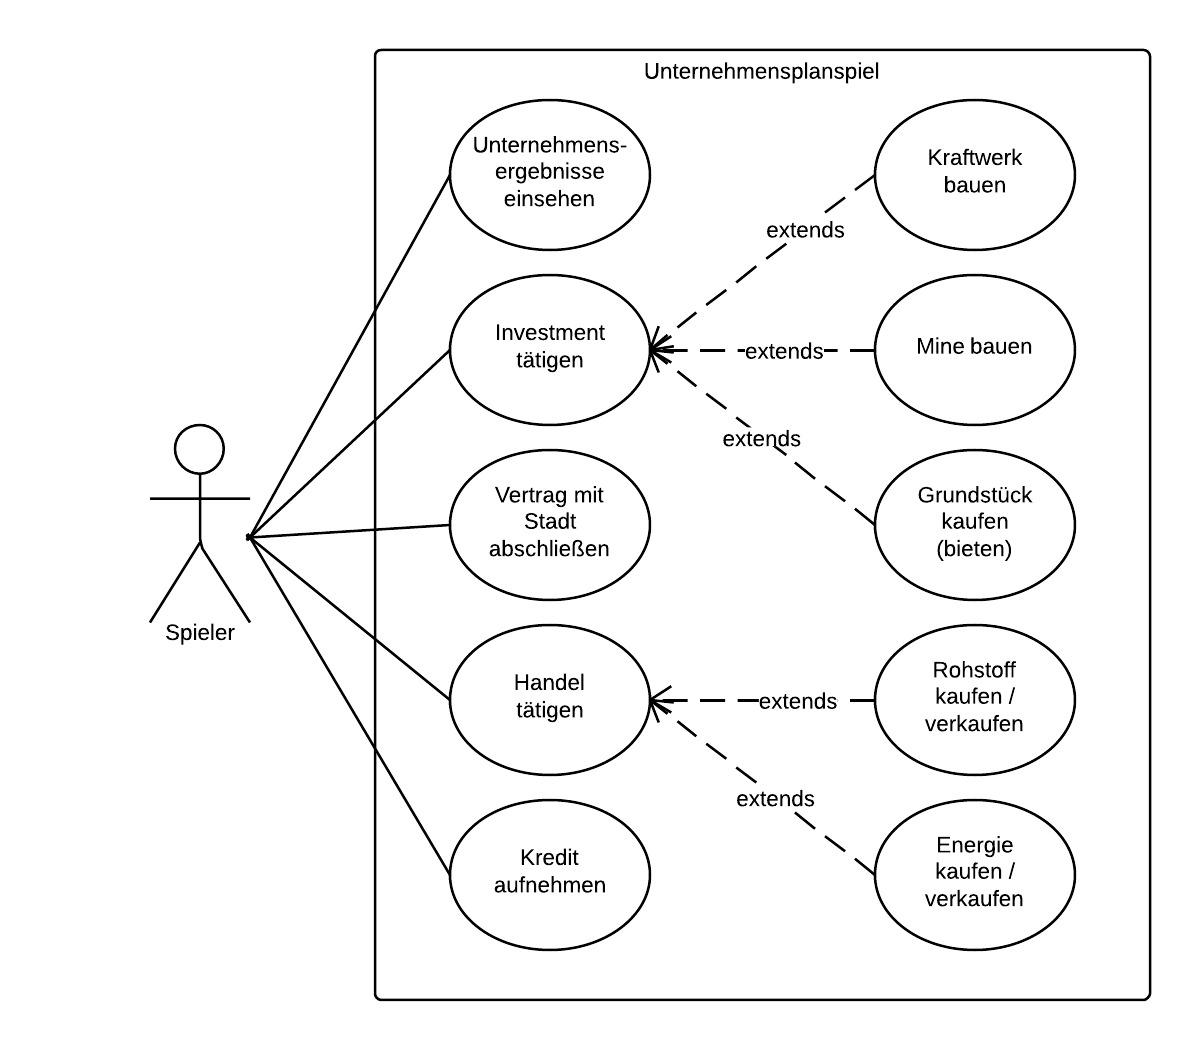
\includegraphics[width=0.8\textwidth]{se-wa-jpg/usecase}
\caption{Use Case Diagramm}
\label{Use Case Diagramm}
\end{figure}
%Olli
\section{Architektur}
In diesem Kapitel wird die Software Architektur des Projektes vorgestellt. Das
Spiel wurde nach dem ``MVC'' (Model View Controller) Konzept entwickelt. Das bedeutet,
dass die Klassen, die das Modell und dessen Daten darstellen, sowohl das View
als auch den Controller nicht kennen. Das View, das in diesem Fall die
graphische Benutzeroberfl�che ist kennt hingegen zwar das Modell, den
Controller aber nicht. Diese Trennung ist wichtig, damit die Datenhaltung und
Logik seperat von der graphischen Benutzeroberfl�che entwickelt werden kann.

Der Controller kennt beide anderen Ebenenen und
verwaltet diese --- es sorgt beispielsweise daf�r, dass die Benutzeroberfl�che
immer die aktuellen Daten anzeigt. In unserem Projekt wird der Controller durch
eine einzelne Klasse gebildet, die das Singleton Pattern implementiert. Dadurch
kann jede Klasse statisch auf den Controller zugreifen, ohne eine Referenz zu
ihm speichern zu m�ssen --- und trotzdem kann der Controller objektorientiert
entwickelt werden. %Das hier eher = Implementierung?

%MVC Bild
\begin{figure}[H]
\centering
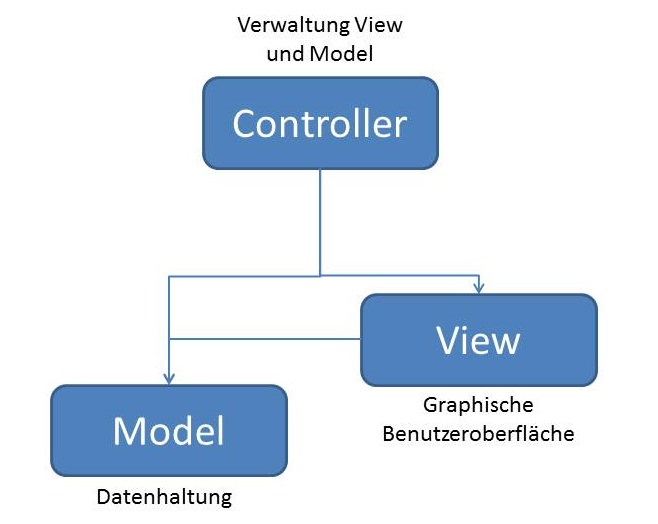
\includegraphics[width=0.5\textwidth]{se-wa-jpg/mvc}
\caption{Model View Controller Konzept}
\label{MVC Konzept}
\end{figure}


Es wurde fr�h entschieden, dass das Spiel nicht nur auf einem Computer
laufen soll (``Hotseat''), sondern dass das Spiel von einem Server kontrolliert
wird und die Daten an Clients, die auf unterschiedlichen Computern
laufen k�nnen, verschickt werden --- somit k�nnen die Spieler gleichzeitig
spielen und haben keine langen Wartephasen. Die Logik des Spiels und die
Datenhaltung befinden sich verteilt auf dem Server und auf den einzelnen
Clients. Der Server verwaltet die wichtigsten Daten, die allen Clients bekannt
sein m�ssen (beispielsweise das Spielfeld und Informationen dar�ber) w�hrend auf
den Clients zum Beispiel die finanziellen Daten wie die Bilanz gehalten
werden.

Des Weiteren wurde keine persistente Speicherung der Spieldaten vorgesehen.
Sobald der Server also nicht mehr l�uft sind die Daten des aktuellen Spiels
verloren. Dies reduziert die Komplexit�t des Modells, denn es muss beim
Initialisieren des Spiels keine Daten laden und beim Beenden des Spiels keine
Daten speichern.


\newpage
\section{OOA-Klassenmodell}

Im Folgenden wird unser, auf Basis der Anforderungen unseres Planspiels,
erstelltes Klassendiagramm der Analysephase aus \ref{OOA-Client} und
\ref{OOA-Server} auf \pageref{OOA-Client} und \pageref{OOA-Server} n�her
erl�utert. 

Das Klassendiagramm ist in zwei H�lften aufgeteilt. In dem ersten Teil werden
die Klassen f�r den Clienten und die Klassen, die f�r die r�ndliche Kommunikation
zwischen Server und Client genutzt werden, abgebildet. Der zweite Teil enth�lt
die Klassen des Servers und Klassen und Interfaces, die f�r die
au�erordentliche Kommunikation zwischen Server und Client vorgesehen sind.

Das Herzst�ck des Unternehmens, dass auf Client-Seite vorgesehen ist, ist die
'Company' -Klasse. In ihr werden alle Entscheidungen des Spielers bearbeitet
und sie enth�lt alle Informationen, die der Spieler �ber sein Unternehmen
ben�tigt.
Dies sind die Mitarbeiter, die einzelnen Abteilungen und die Beziehungen, die zu
den einzelnen Regionen bestehen.

In den Beziehungen zu den Regionen werden entweder in einer 'ResourceRelation'
der Besitztum dieser Region erlangt und, sollte man schon eine solche Region
besitzen, auch die vorhandenen Geb�ude dieser Region gespeichert. Die
'CityRelation' enth�lt alle Informationen �ber die Bewohner einer Stadt und mit
dem 'Contract' auch �ber die Kunden des Unternehmens.

Die Abteilungen des Unternehmens umfassen das 'Warehouse', das
'InvestmentManagement', den 'Research', die 'Finances' und das 'Marketing'. In
dem Warehouse werden die Rohstoffe gelagert, die in Minen produziert
werden und die f�r die Produktion von Strom in den Kraftwerken ben�tigt werden.
Auch gehandelter Rohstoffe werden hier entnommen oder eingelagert.\\
Das InvestmentMangement beinhaltet alle Geb�ude (Minen und Kraftwerke) und alle
Grundst�cke (Regionen), die das Unternehmen besitzt. Hier werden neue Geb�ude
hinzugef�gt, Abschreibungen berechnet und Produktionsmengen eingestellt und
ausgelesen. Zudem besitzt jedes Kraftwerk mehrere 'PowerStationRelation', die
beinhaltet wieviel Energie das Kraftwerk den einzelnen, umliegenden St�dten
liefert. Diese Beziehung von einem Kraftwerk zu den St�dten ist vorgesehen,
damit die gewollte, maximale Lieferentfernung von drei Feldern nicht
�berschritten wird.\\
Die 'Finances' sind vorgesehen, um alle vier Quartale eine Bilanz und eine
Gewinn und Verlustrechnung aufzustellen. Alle Einnahmen und Ausgaben werden hier
eingespeichert und aufbereitet.\\
Das 'Marketing' ist vorgesehen um die Beliebtheit und die Bekanntheit
bei den Kunden zu beeinflussen.\\
Der letzte Bereich, der 'Research', ist vorgesehen um m�glicherweise eine aktive
Forschung einbauen zu k�nnen. Auf Grund von anderen Priorit�ten ist dieser aber 
nicht weiter modelliert und auch nicht in das entg�ltige Planspiel aufgenommen
worden.

Die Verbindung zwischen Client und Server wird aufgebaut indem sich der Client
�ber die 'Client'-Klasse mit der 'Server'-Klasse auf Serverseite verbindet. Dort
wird die Verbindung akzeptiert und nach dem 'Thread-per-Connection'-Prinzip ein,
f�r jeden Clienten seperater Thread der Klasse 'Connection' erstellt.

Die anschlie�ende Kommunikation wird mit Objekten, die jeweils das
'Messagable'-Interface implementieren durchgef�hrt. So kann jede beliebige
Klasse �bertragen werden. Der Empf�nger des Objektes kann nun den MessageType
des Objektes abfragen und wei� somit, wie er mit dem Objekt weiter verfahren
soll. Hierf�r sind spezielle Typen f�r jede unterschiedliche Nachricht, die
kommuniziert werden soll, in zwei Enumerates definiert.

�ber den Server werden jede Runde, alle Entscheidungen der Spieler abgewickelt,
die nicht nur den Spieler selbst, sondern auch andere Spieler betreffen. Vor
allem sind dies, Grundst�cksgebote und -k�ufe und Vertragseinstellungen mit
einer Stadt, nach denen die Kunden des Spielers bestimmt werden. Auch bereits
gebaute Geb�ude werden dem Server mitgeteilt, so dass sie f�r jeden Spieler
ersichtlich werden.

Diese �nderungen werden dem Clienten zu jedem Rundenbeginn �ber das
'Map'-Objekt und die 'CityRelation' mitgeteilt.



\begin{figure}
\centering
\centering
\hspace*{-30mm}
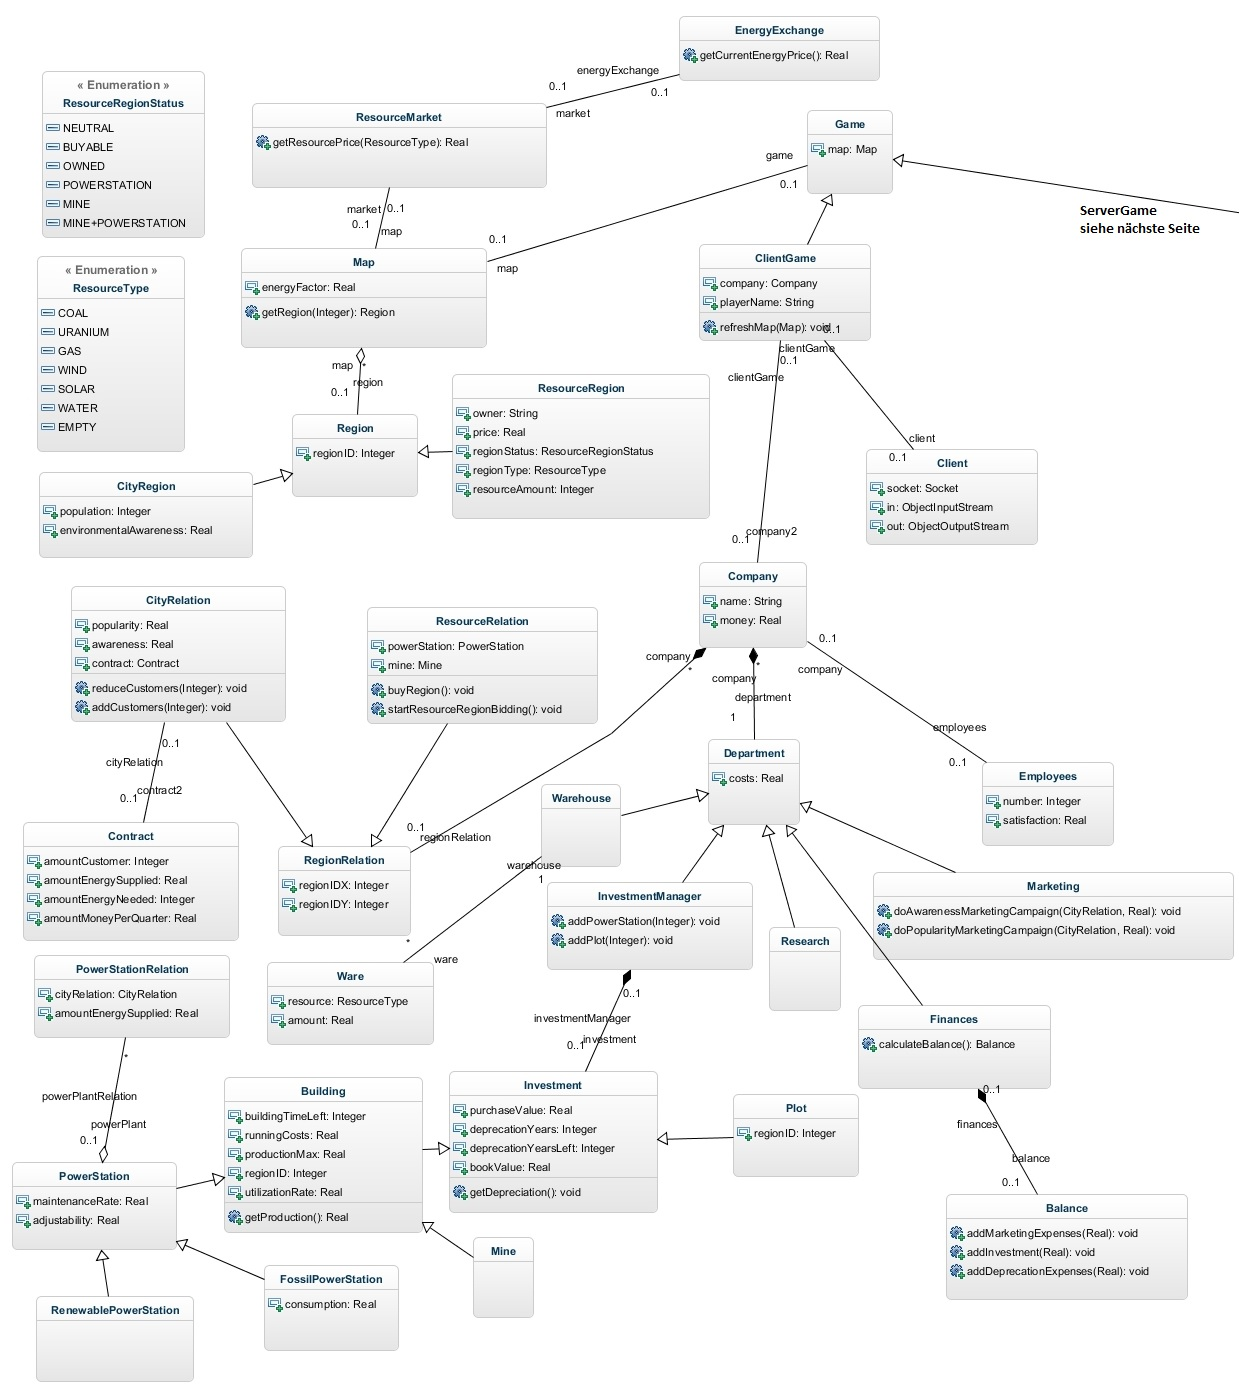
\includegraphics[width=1.3\textwidth]{se-wa-jpg/Client}
\caption{Klassendiagramm Teil 1}
\label{OOA-Client}
\end{figure}
%Die Grafik in Abbildung 
%\ref{labelname} auf Seite \pageref{labelname} ..
\begin{figure}
\centering
\centering
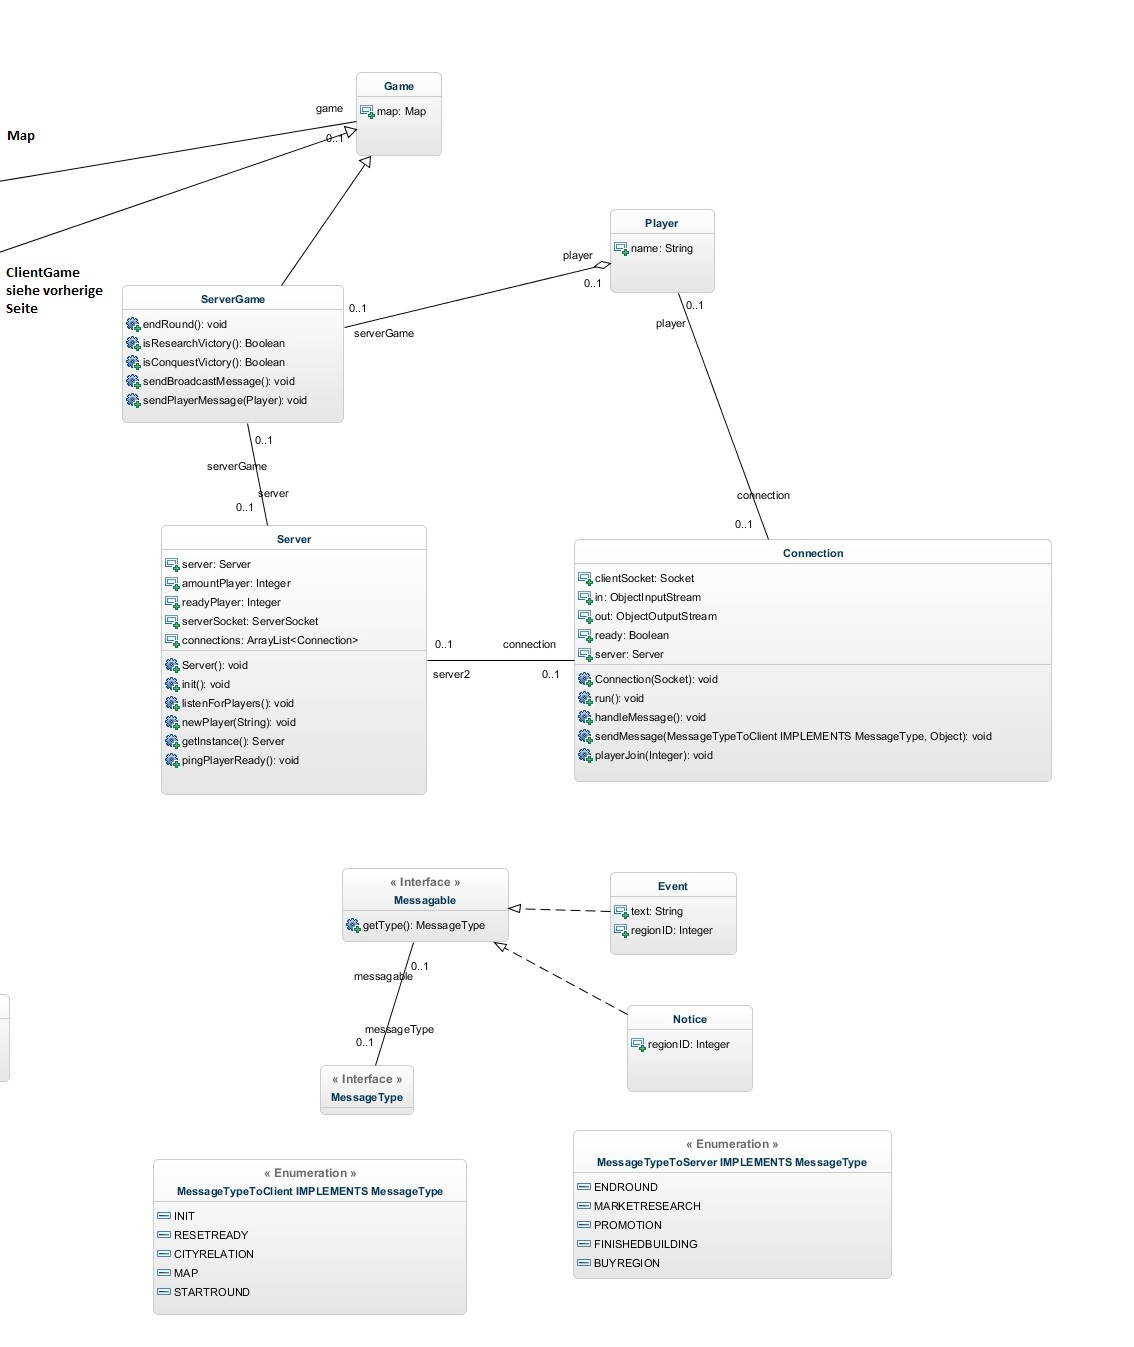
\includegraphics[width=1.1\textwidth]{se-wa-jpg/Server}
\caption{Klassendiagramm Teil 2}
\label{OOA-Server}
\end{figure} %OOA
%Olli
\section{Optimierung}\label{Opt}\label{olli:optimierung}
In diesem Teil der Arbeit wird die Optimierung der Kraftwerksverteilung
erl�utert. Dies wird auf der Seite des Clients ausgef�hrt --- dadurch wird die
Komplexit�t des Algorithmus reduziert, da die Daten des Servers nicht mit denen 
des Clients synchronisiert werden m�ssen. Aus Spielgr�nden wurde entschieden, 
dass sich der Spieler nicht selbst um die Optimierung der Kraftwerke k�mmern 
muss, sondern dass die Optimierung mithilfe des Simplexalgorithmus durchgef�hrt 
wird, da die Kraftwerksverteilung durch ein lineares Optimierungsproblem
formuliert werden kann (\seCite{vgl.}{}{holey}).

Zun�chst das Problem folgenderma�en dargestellt werden: \\
$k$ Kraftwerke mit einer Produktion von $k_i$ haben je $x$ Verbindungen zu $s$
St�dten mit je $y$ Verbindungen, einem Preis $p$ und einem Bedarf $n$. Dabei wird eine Verbindung nur gebildet,
wenn der Spieler mit der jeweiligen Stadt einen Vertrag besitzt und das
Kraftwerk  h�chstens drei Felder von der Stadt entfernt ist. So k�nnte 
beispielsweise folgendes Optimierungsproblem entstehen:

%Bild Optimierung
\begin{figure}[H]
\centering
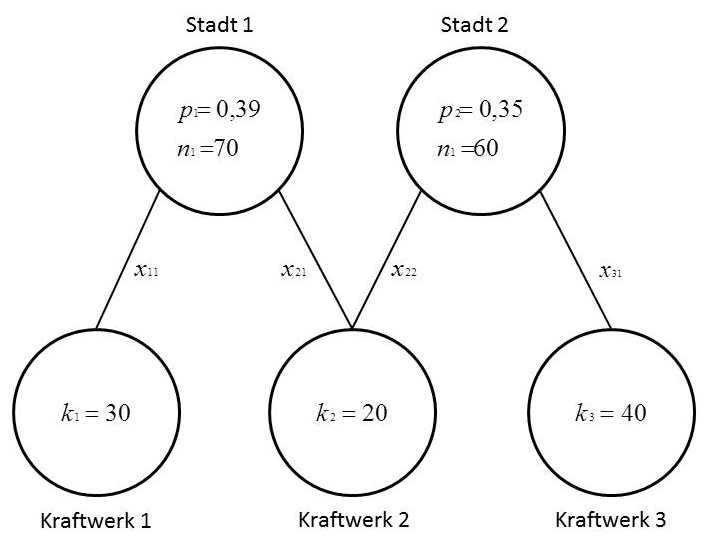
\includegraphics[width=0.85\textwidth]{se-wa-jpg/optimizing}
\caption{Beispiel f�r ein Optimierungsproblem}
\label{Beispielproblem}
\end{figure}

Nach dem Simplexalgorithmus m�ssen f�r dieses Problem nun die Zielfunktion und
die Nebenbedingungen aufgestellt werden. Die Zielfunktion $z$ ist durch die 
Maximierung des Umsatzes gegeben. Dabei ist $p_i$ der Preis der Stadt $i$,
$k_j$ die maximale Produktion des Kraftwerkes $j$ und $y_j$ die Verbindung
zwischen der Stadt und dem Kraftwerk.

\begin{align*}
z &= \sum\limits_{i=1}^s p_i * \sum\limits_{j=1}^y k_j * y_j \\
  &= 0.39 (30 * x_{11} + 20 * x_{21}) + 0.35 (20 * x_{22} + 40 * x_{31})
\end{align*}

Als n�chstes wird f�r jedes Kraftwerk eine Nebenbedingung erstellt. Die
Verteilung der Produktion eines Kraftwerkes ist durch mehrere
Variablen $x_i$ gegeben (pro Kraftwerkverbindung eine).
Addiert d�rfen diese h�chstens $1$ sein, damit das Kraftwerk nicht mehr auf die
Verbindungen verteilt, als es eigentlich maximal produzieren kann:

\begin{align*}
g: &\sum\limits_{i=1}^x x_i &\leq 1 \\
g_1: &x_{11} &\leq 1 \\
g_2: &x_{21} + x_{22} &\leq 1 \\
g_3: &x_{31} &\leq 1
\end{align*}

Anschlie�end wird f�r jede Stadt eine Nebenbedingung erstellt, in der der
maximale Bedarf $n$ der Stadt gepr�ft wird. $y$ ist hier die Anzahl der Verbindungen der
Stadt und $k_j$ die Produktion des Kraftwerkes $j$:

\begin{align*}
g: \sum\limits_{j=1}^y y_j * k_j \leq n \\
g_4: 30x_{11} + 20x_{21} \leq 50 \\
g_5: 20x_{22} + 40x_{31} \leq 60
\end{align*}

Danach werden die Zielfunktion und die Nebenbedingungen in die Normalform
gebracht. In diesem Fall werden in den Nebenbedingungen nur Schl�pfvariablen
angelegt und als Startl�sung die Kraftwerksverbindungsvariablen $x_i = 0$
gesetzt. Darauffolgend werden nach dem Simplexalgorithmus die Daten in eine
Matrix eingef�gt:

\begin{align*}
\begin{array}{ c | c | c | c | c | c | c | c | c | c | c }
BV & x_{11} & x_{21} & x_{22} & x_{31} & s_1 & s_2 & s_3 & s_4 & s_5 & b \\
\hline
s_1 & 1 & 0 & 0 & 0 & 1 & 0 & 0 & 0 & 0 & 1 \\ 
s_2 & 0 & 1 & 1 & 0 & 0 & 1 & 0 & 0 & 0 & 1 \\
s_3 & 0 & 0 & 0 & 1 & 0 & 0 & 1 & 0 & 0 & 1 \\
s_4 & 30 & 20 & 0 & 0 & 0 & 0 & 0 & 1 & 0 & 50 \\
s_5 & 0 & 0 & 20 & 40 & 0 & 0 & 0 & 0 & 1 & 60 \\
\hline
z & -0.39*30 & -0.39*20 & -0.35*20 & -0.35*40 & 0 & 0 & 0 & 0 & 0 & 0
\end{array}
\end{align*}

Nach mehreren Iterationsschritten zeigt sich folgende L�sung als optimal:

\begin{align*}
x_{11} &= 1 & s_1 &= 0 \\
x_{21} &= 1 & s_2 &= 0 \\
x_{22} &= 0 & s_3 &= 0 \\
x_{31} &= 1 & s_4 &= 0 \\
& & s_5 &= 20
\end{align*}

Die Stadt $s_1$ wird aufgrund des h�heren Preises vom Kraftwerk $k_2$ bevorzugt
und wird deswegen �ber die Verbindung $x_{21} = 1$ beliefert. $x_{22} = 0$
bedeutet, dass $k_2$ zwar an Stadt $s_2$ liefern k�nnte, es aber nicht macht. Die
Schl�pfvariablen $s_{1\ldots3} = 0$ bedeutet, dass alle Kraftwerke ihre
komplette Produktion nutzen. Zuletzt bedeutet $s_4 = 0$, dass der Bedarf von
Stadt $s_1$ komplett gef�llt wird und $s_5 = 20$, dass der Stadt $s_2$ noch
$20$ Einheiten fehlen.




%Olli
\section{Vertr�ge}\label{olli:vertraege}
Ein wichtiger Teil des Spieles ist f�r den Benutzer das Abschlie�en von
Vertr�gen mit St�dten. Dabei soll zwischen den Spielern eine Konkurrenz
entstehen, um einen Bezug zur Realit�t herzustellen. Dieser
Algorithmus wird jede Runde erneut durchlaufen, damit eine Preiskonkurrenz
zwischen Spielern entsteht --- zudem kann sich dadurch die Anzahl der Kunden
�ndern, ohne dass der Spieler Werte �ndert. Bevor der Algorithmus durchgef�hrt
wird, werden alle bestehenden Vertr�ge mit der Stadt nach ihrem Preis
aufsteigend geordnet. Dies hat zur Auswirkung, dass die Preiswahl des Spielers
ausschlaggebend f�r die Anzahl seiner Kunden ist.

Zun�chst wird die Anzahl der Kunden $y_0$ berechnet, die ein Spieler bei dem
durchschnittlichen Preis bei seiner Bekanntheit und Beliebtheit erhalten w�rde. 
$$y_0 = Bekanntheit * Beliebtheit * Population$$
Anschlie�end wird diese Variable der ``Standardkunden'' $y_0$ in eine
quadratische Funktion gegeben. Diese Parabel hat einen Sattelpunkt, der
sich bei $S(x_d/y_0)$ befindet, wobei $x_d$ der Durchschnittspreis der Stadt
representiert. Ist der Preis des Spielers also unter dem Durchschnittspreis,
werden ihm entsprechend mehr und mehr (quadratisch steigend) Kunden zugewiesen 
--- ist der Preis des Spielers unter dem Durchschnittspreis werden ihm umgekehrt
weniger Kunden als $y_0$ zugewiesen. Werden dem Spieler durch diese Funktion $y
= 0$ Kunden zugewiesen, wird der Algorithmus hier abgebrochen und der Spieler  
erh�lt keinen Vertrag mit der Stadt bzw. sein aktueller Vertrag wird gek�ndigt. 

%Bild Paralbel

Durch die Wahl einer quadratischen Funktion sind Preisabweichungen sehr
entscheidend --- anders als bei anderen Produkten und M�rkten ist in dem
Energiemarkt der Preis wichtiger als die Bekanntheit und Beliebtheit einer
Firma. 

Nun werden zwei weitere Bedingungen gepr�ft: \\
Der Spieler kann die maximale Energie festlegen, die er f�r den Vertrag
bereitstellen m�chte. Wird dieser Wert �berschritten, erh�lt er maximal so viele
Kunden, wie er beliefern kann.\\
Zuletzt muss �berpr�ft werden, ob noch genug freie Kunden in der Stadt
vorhanden sind --- es k�nnte also beispielsweise sein, dass der Spieler durch
die Preiswahl anderer Spieler aus diesem Grund keine Kunden mehr erh�lt.

\newpage
\chapter{Implementierung}
%Matthias
\section{Projektablauf Matthias}
%J�rn
\section{Fachkonzept}
Im \ref{ooa} wurde bereits das Klassendiagramm der Analysephase n�her erl�utert.
Bei der Implementierung auf Basis dieses Klassenmodells haben wir aber noch
einige �nderungen und Einschr�nkungen vorgenommen. Im folgenden Abschnitt werden
diese Unterschiede und dessen Hintergr�nde n�her erl�utert.

Durch Priorit�ten die wir in der Entwurfsphase ges�tzt haben, sind gegen�ber dem
OOA-Diagramm auch einige Bereiche weggefallen:
\begin{itemize}
  \item {\textbf{Marketing}}\\
  Das Marketing und die dazugeh�rige Marktforschung und Werbung haben zeitlich
  nicht mehr in den Plan gepasst.
  \item{\textbf{Mitarbeiter}}\\
  Die Mitarbeiter als einzelnes Objekt zu modellieren erschien uns im Laufe der
  Entwurfsphase in einem Geb�udeintensiven Unternehmen f�r keine Notwendigkeit
  mehr. Deswegen haben wir uns nun dazu entschieden auf eine Mitarbeiteranzahl
  und weiteres zu verzichten und diese vielmehr in die laufenden Kosten der
  einzelnen Kraftwerke mit einflie�en zu lassen.
\end{itemize}



\subsection{Client-Server}


\begin{figure}
\centering
\centering
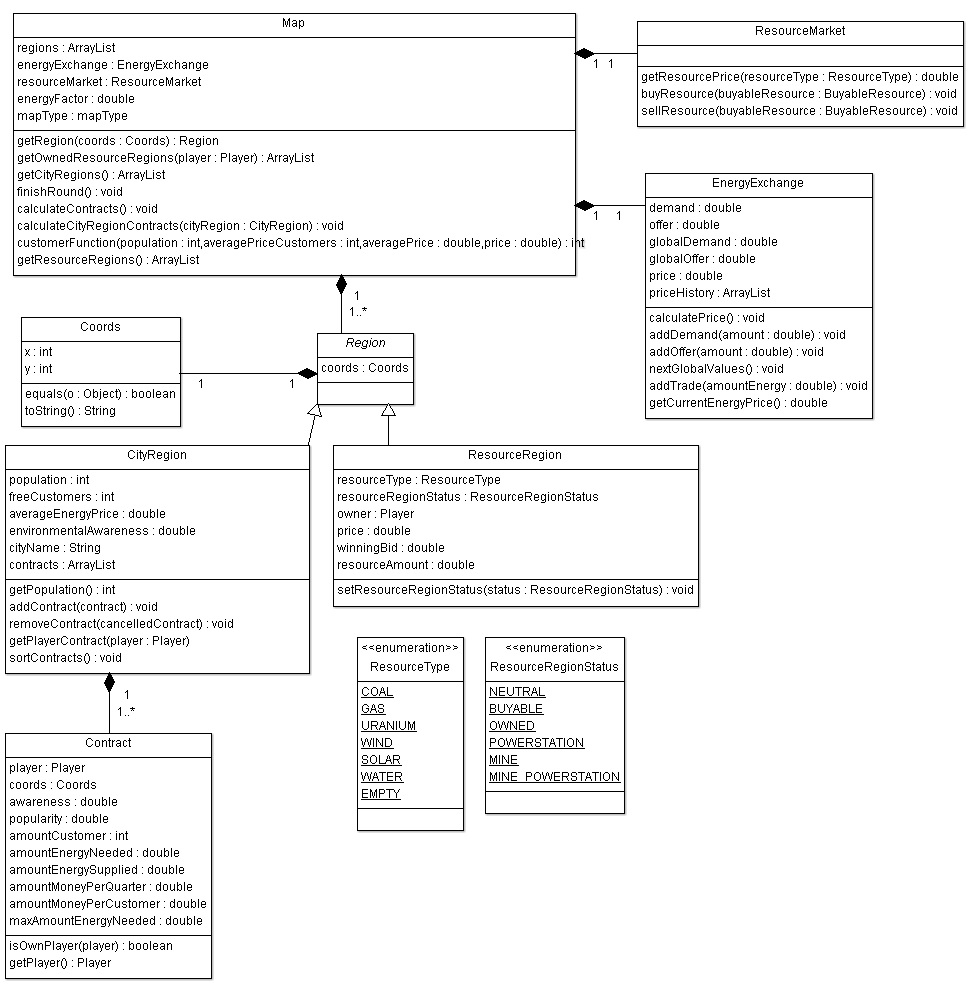
\includegraphics[width=1.1\textwidth]{se-wa-jpg/OOD-Map}
\caption{Klassendiagramm Kommunikationsklassen}
\label{OOD-Map}
\end{figure}

Die Client-Server Architektur, die bei unserem Planspiel angewandt wird,
erm�glicht es mehreren Spielern ihren Spielzug gleichzeitig zu absolvieren.
Zwar verringert dies die Wartezeiten der Spieler im Gegensatz zum
Hotseat-Modell, allerdings muss bei einem gemeinsamen Server und mehreren
Clienten darauf geachtet werden, dass es zu keinen Dateninkonsistenzen kommt.
An der ``Thread-per-Connection''-Methode hat sich seit der Analysephase (siehe
\ref{ooa}) nichts ge�ndert, weswegen hier darauf nicht n�her eingegangen wird.

In \ref{OOD-Map} ist die Klassenstruktur abgebildet, die alle Daten enth�lt, die
f�r alle Spieler interessant sind und indirekt auch von diesen ge�ndert werden
k�nnen. Hierbei haben wir uns dazu entschlossen nicht alle Entscheidungen des
Spielers dem Server mitzuteilen, sondern einige Eingaben auf Client-Seite
zu bearbeiten, um den Server nicht unn�tig zu belasten und den
Datenverkehr zu vermindern. Zum Beispiel wird das Verm�gen eines Unternehmens
komplett auf Client-Seite bearbeitet, da es f�r die anderen Spieler im Spiel
nicht sichtbar gemacht werden soll.\\
Um Dateninkonsistenz zu vermeiden werden alle �nderungen, die alle Spieler
betreffen, direkt an den Server gesendet, dieser wertet die �nderungen aus
�bertr�gt sie gegebenenfalls in den entsprechenden Objekte. Zu Rundenbeginn
wird nun die gesamt Objektstruktur, die in einem Objekt der 'Map'-Klasse auf
Serverseite gespeichert ist, an alle Clients �bertragen. Dadurch, dass nur der
Server solche �nderungen vornehmen kann und diese auch nicht von verschiedenen
'Connection'-Threads gleichzeitig vorgenommen k�nnen (``Synchronized''), wird
die richtige Datenhaltung sichergestellt.

W�hrend der Analysephase war es angedacht, Vertr�ge mit einer Stadt unabh�ngig
vom Rundenende zu schlie�en. Diese Idee wurde w�hrend der Entwcklung verworfen,
so dass nun jeder Spieler seine Vertragsvorschl�ge dem Server w�hrend der Runde
zusendet, der Server nach der Runde die Kunden jedes Spielers
errechnet und zum n�chsten Rundenanfang diese den Spielern mitteilt.\\
Wie in \ref{OOD-Map} zu sehen ist, haben wir uns deswegen dazu entschieden den
'Contract', der vorher unter dem Unternehmen in dem Bereich der Beziehungen zu
den Regionen angeordnet war, nun der 'Map' und darin der 'CityRegion' zu
unterordnen.\\
Diese �nderung in der Struktur der Fachlogik erlaubt es dem Server weiterhin,
alle Daten, die jede Runde den Spielern zugeschickt werden, in einer einzigen
Objektstruktur zu �bertragen.
Dies erm�glicht zum einen eine einfache Kommunikation vom Server zum Client und
zum anderen kann nun auch der Client alle wichtigen �nderungen der Runde aus
einem einzigen Objekt auslesen, in dem er die neu erhaltene 'Map' mit der
vorhandenen aus der vergangenen Runde vergleicht.

Im folgenden werden die einzelnen Klassen, die vom Server zu dem Client
�bertragen werden, n�her erl�utert:
\begin{itemize}
  \item {\textbf{Klasse Map}}\\
  Die Klasse Map enth�lt zum Einen alle Regionen der Spielkarte, die zu Beginn
  des Spiels vom Server generiert werden und zum Anderen die
  Stromb�rse('EnergyExchange') und den Ressourcenmarkt. Au�erdem werden in ihr
  die Kunden der einzlnen Spieler in den verschiedenen St�dten berechnet.
  \item{\textbf{Klasse RessourceMarket}}\\
  Der Ressourcenmarkt setzt sich aus den drei unterschiedlichen Rohstoffen
  zusammen, die in unserem SPiel vorhanden sind. Die Preise f�r die Rohstoffe
  sind in dem Programm als Konstanten festgesetzt und �ndern sich nicht mit der
  Zeit.
  \item{\textbf{Klasse EnergyExchange}}\\
  Die Stromb�rse im Spiel hat einen schwankenden Preis. Dieser reguliert sich
  aus Angebot und Nachfrage. Jedes mal wenn ein Spieler einen Stromhandel
  abschlie�t, schickt der Client eine kleine Nachricht �ber die h�he des Handels
  an den Server, der daraufhin den neuen Preis f�r die n�chste Runde berechnet.
  \item{\textbf{Klasse Region und Klasse Coords}}\\
  Die Klasse Region ist daf�r gedacht, dass sie mit ihren Koordinaten, die in
  der Klasse Coords gespeichert sind, eindeutig ermittelt werden kann. Die
  Region ist nich daf�r gedacht, dass sie f�r sich instanziiert wird, sondern
  mit Hilfe von Vererbung entweder als Ressourcenregion oder Stadtregion benutzt
  wird.
  \item{\textbf{Klasse CityRegion und Klasse Contract}}\\
  Die Stadtregion enth�lt alle Informationen �ber die Einwohner der Stadt und
  die Vertr�ge mit den verschiedenen Energielieferanten. Die Stadt wird mit
  einer Einwohnerzahl und verschiedenen Kennziffern zum Spielstart generiert,
  w�hrend die Kundenzahlen, die in den Contracts gespeichert sind, sich jede
  Runde durch Preis�nderungen der Spieler �ndern k�nnen. Jede Stadt hat f�r
  jedes Unternehmen, dass in ihr Kunden besitzt, ein seperates Contract-Objekt.
  \item{\textbf{Klasse RessourceRegion}}\\
  Die RessourceRegion wird mit einem bestimmten RessourceType (siehe
  Enumeration RessouurceType) und gegebenenfalls einer Menge des Rohstoffes zum
  Spielstart generiert. F�r erneuerbare Energien, wie z.B. Wasser entf�llt
  nat�rlich die Rohstoffmenge. W�hrend des Spiels k�nnen Spieler auf die
  Regionen bieten, um sie bebauen zu k�nnen. Diese Gebote werden an den Server
  gesendet, der dann den Zuschlag an ein Unternehmen gibt, der danach zum
  Besitzer der Region wird. Zudem meldet der Besitzer der Region dem Server,
  sobald er ein Geb�ude in einer Region fertiggestellt hat. Dieser schreibt dies
  dann in das Region-Objekt, sodass dies auch f�r die anderen Spieler sichtbar
  wird.
  
\end{itemize}


\subsection{Geb�ude}



PowerstatioNrelation stellt die verbindung zwischen einem Kraftwerk und einer
Stadt mit Vertrag da \ref{Opt} 

%Marco
\section{Design}\label{marco:design}
Die Benutzeroberfl�che ist eines der wichtigsten Bestandteile eines Spieles. Dadurch wird dem Spieler ein echtes Spielerlebnis geboten, wobei jegliche Spielinformationen strukturiert abgebildet werden. Auf den folgenden Seiten wird der Entwicklungsprozess, als auch die Ergebnisse und m�gliche Verbesserungsm�glichkeiten dargelegt und wiedergegeben.
Die Entwicklung des Designs spielt eine wichtige Rolle, welche sich in einzelne Phasen unterteilen lassen kann. Die einzelnen Phasen, Schritte und Ideen dahinter werden im Folgenden dargelegt.

\subsection{Brainstorming \& erste Skizzen}
Nach der Entwicklung des Spielkonzeptes und der Programmierung der ersten
Spielfunktionen wurde damit begonnen die ersten Ideen f�r das User-Interface zu
sammeln. Dazu wurde eine gemeinsame Brainstorming-Session gestartet und alle
m�glichen Vorschl�ge zusammengetragen. Diese Vorschl�ge wurden dann in erste
Skizzen verpackt und m�gliche Anordnungen und Elemente diskutiert. Da die Skizzen jedoch sehr einfach, un�bersichtlich und ungenau waren, wurden daraus, mit Hilfe von Grafikprogrammen, Mockups erstellt, um die Ideen realit�tsgetreu darzustellen und  wirken zu lassen und somit sowohl St�rken als auch Schw�chen der Ideen aufzudecken und diese zu optimieren.

\subsection{Mockup \& Ideen}
Im Folgenden werden die einzelnen Mockup-Grafiken dargestellt und kurz Erl�utert, um unsere Ideen der grafischen Aufteilung genau zu beschreiben.

\subsubsection{Elemente}
Um den Spieler nicht zu verwirren wird auf statische Oberfl�chenelemente gesetzt, welche sich in jedem Bildschirm an denselben Stellen befinden. Daf�r wurde der Bildschirm der Mockups in drei Teile geteilt:
\begin{itemize}
\item Men�leiste
\item Hauptframe
\item Sidebar
\end{itemize}

Die \textbf{Men�leiste} befindet sich am oberen Bildschirmrand und stellt dem Spieler die Navigation auf die unterschiedlichen Seiten zur Verf�gung. Die Hintergrundfarbe ist ein starkes braun.

Im \textbf{Hauptframe} werden die Hauptinformationen des Spiels dargestellt und die Hauptinteraktionen des Spielers ausgef�hrt. Als Hintergrundfarbe wurde ein Beigeton gew�hlt, welche die Farbe von Erde (Sand) widerspiegeln soll.

Die \textbf{Sidebar} dient dabei als Erweiterung des Hauptframes und bietet dem Spieler zus�tzliche Informationen, aber auch Interaktionsm�glichkeiten an.


\subsubsection{Unternehmens�bersicht}
Die Idee hinter der Unternehmens�bersicht ist, dass der Spieler einen �berblick
�ber alle wichtigen Informationen seines Unternehmens bekommt. Dazu z�hlt der Kontostand, Einnahmen, Ausgaben, Anzahl der Rohstoffe, Stromproduktion, Stromverbrauch, Strombilanz und die Anzahl der im Besitz befindenden Kraftwerke und Minen. Des Weiteren soll der Nutzer auf dieser Seite auch �ber Aktionen der vorangegangen Spielrunde informiert werden, um keine wichtigen Interaktionen und Ereignisse zu verpassen. Die einzelnen Informationen werden dabei klassisch als Text dargestellt, um die einzelnen Werte eindeutig und schnell dem Spieler zur Verf�gung zu stellen.

\begin{figure}[H]
\centering
\centering
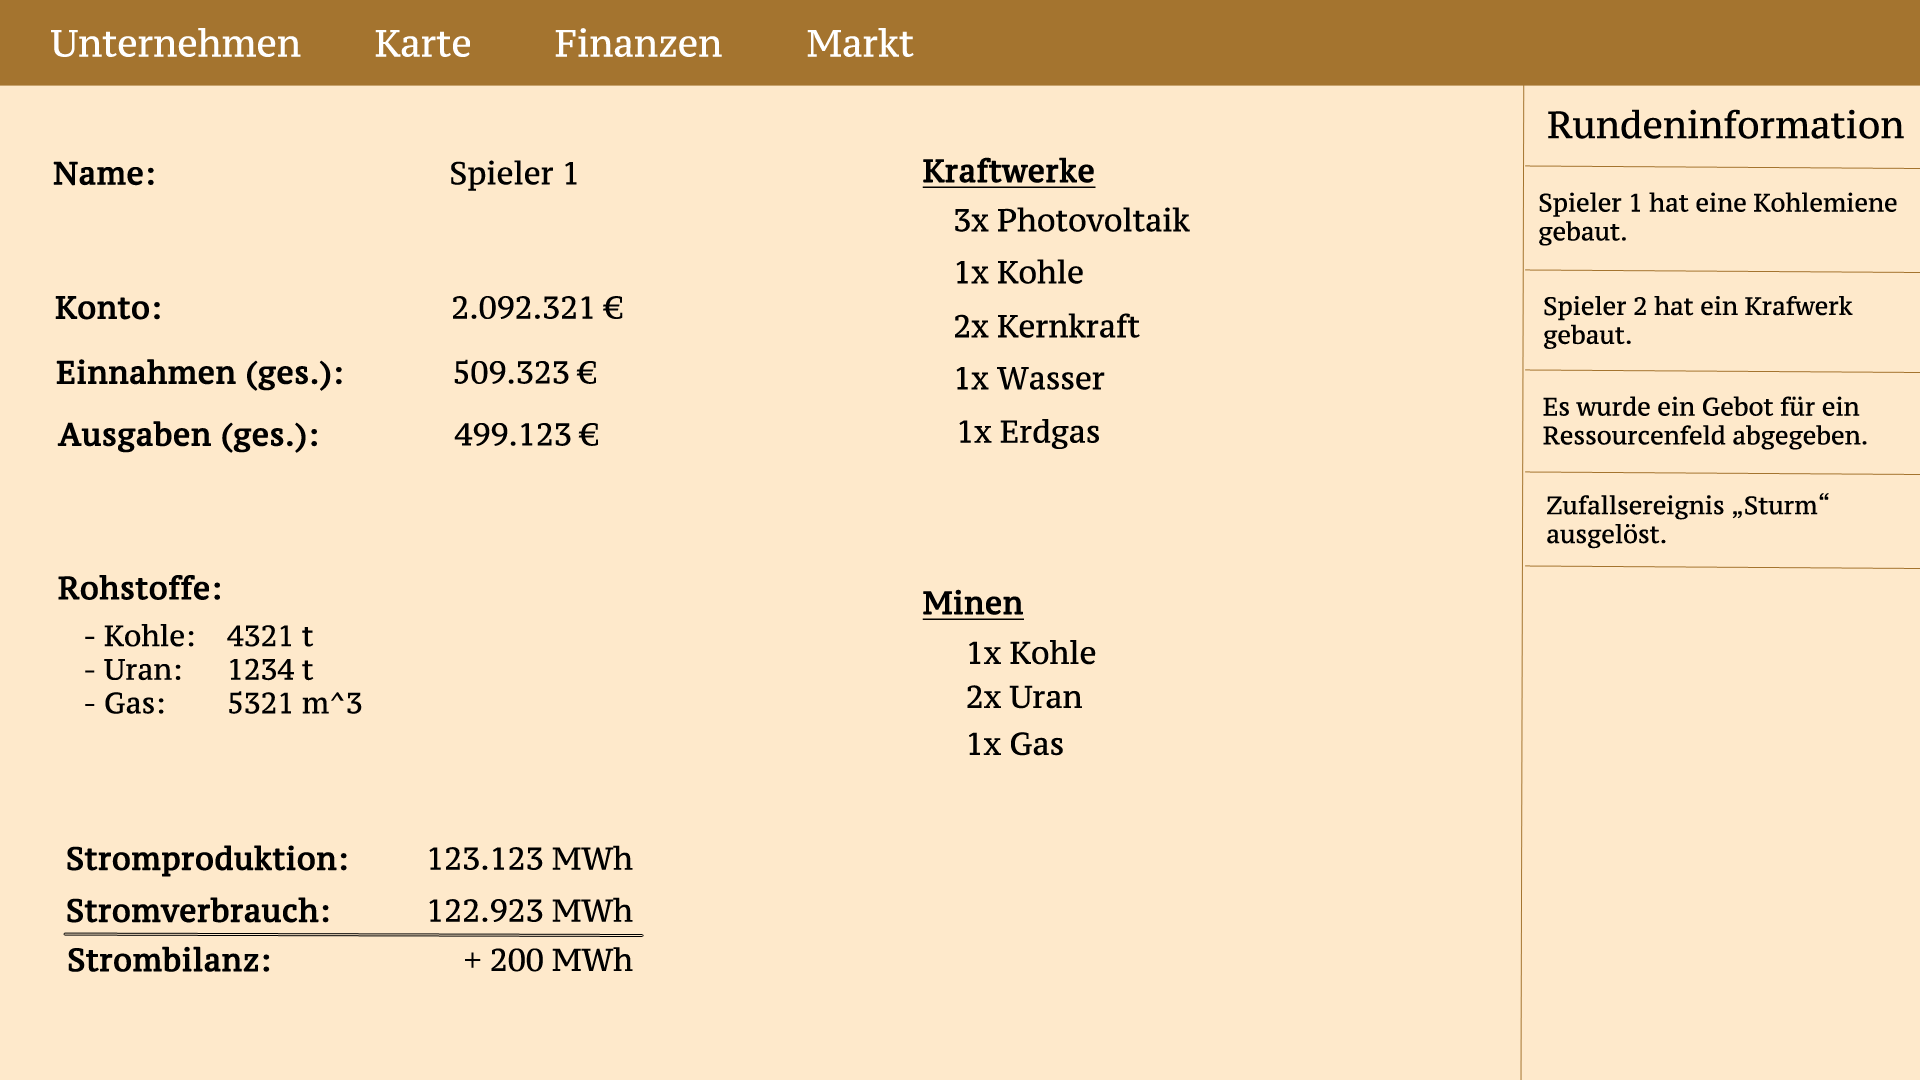
\includegraphics[width=0.9\textwidth]{se-wa-jpg/gui_unternehmen}
\caption{Unternehmens�bersicht}
\label{Unternehmens�bersicht}
\end{figure}

\subsubsection{Karte}
Die Karte stellt den Hauptinteraktionspunkt des Spielers dar und bildet das
Spielfeld ab. Die Form eines Feldes ist ein Hexagon, welches dem Spiel Civilization nachempfunden ist. Dabei wird in drei verschiedene Feldertypen unterschieden:
\begin{itemize}
\item Ressourcen
\item St�dte
\item Leere Felder
\end{itemize}


\subsubsection{Karte mit ausgew�hltem Ressourcenfeld}
\begin{figure}[H]
\centering
\centering
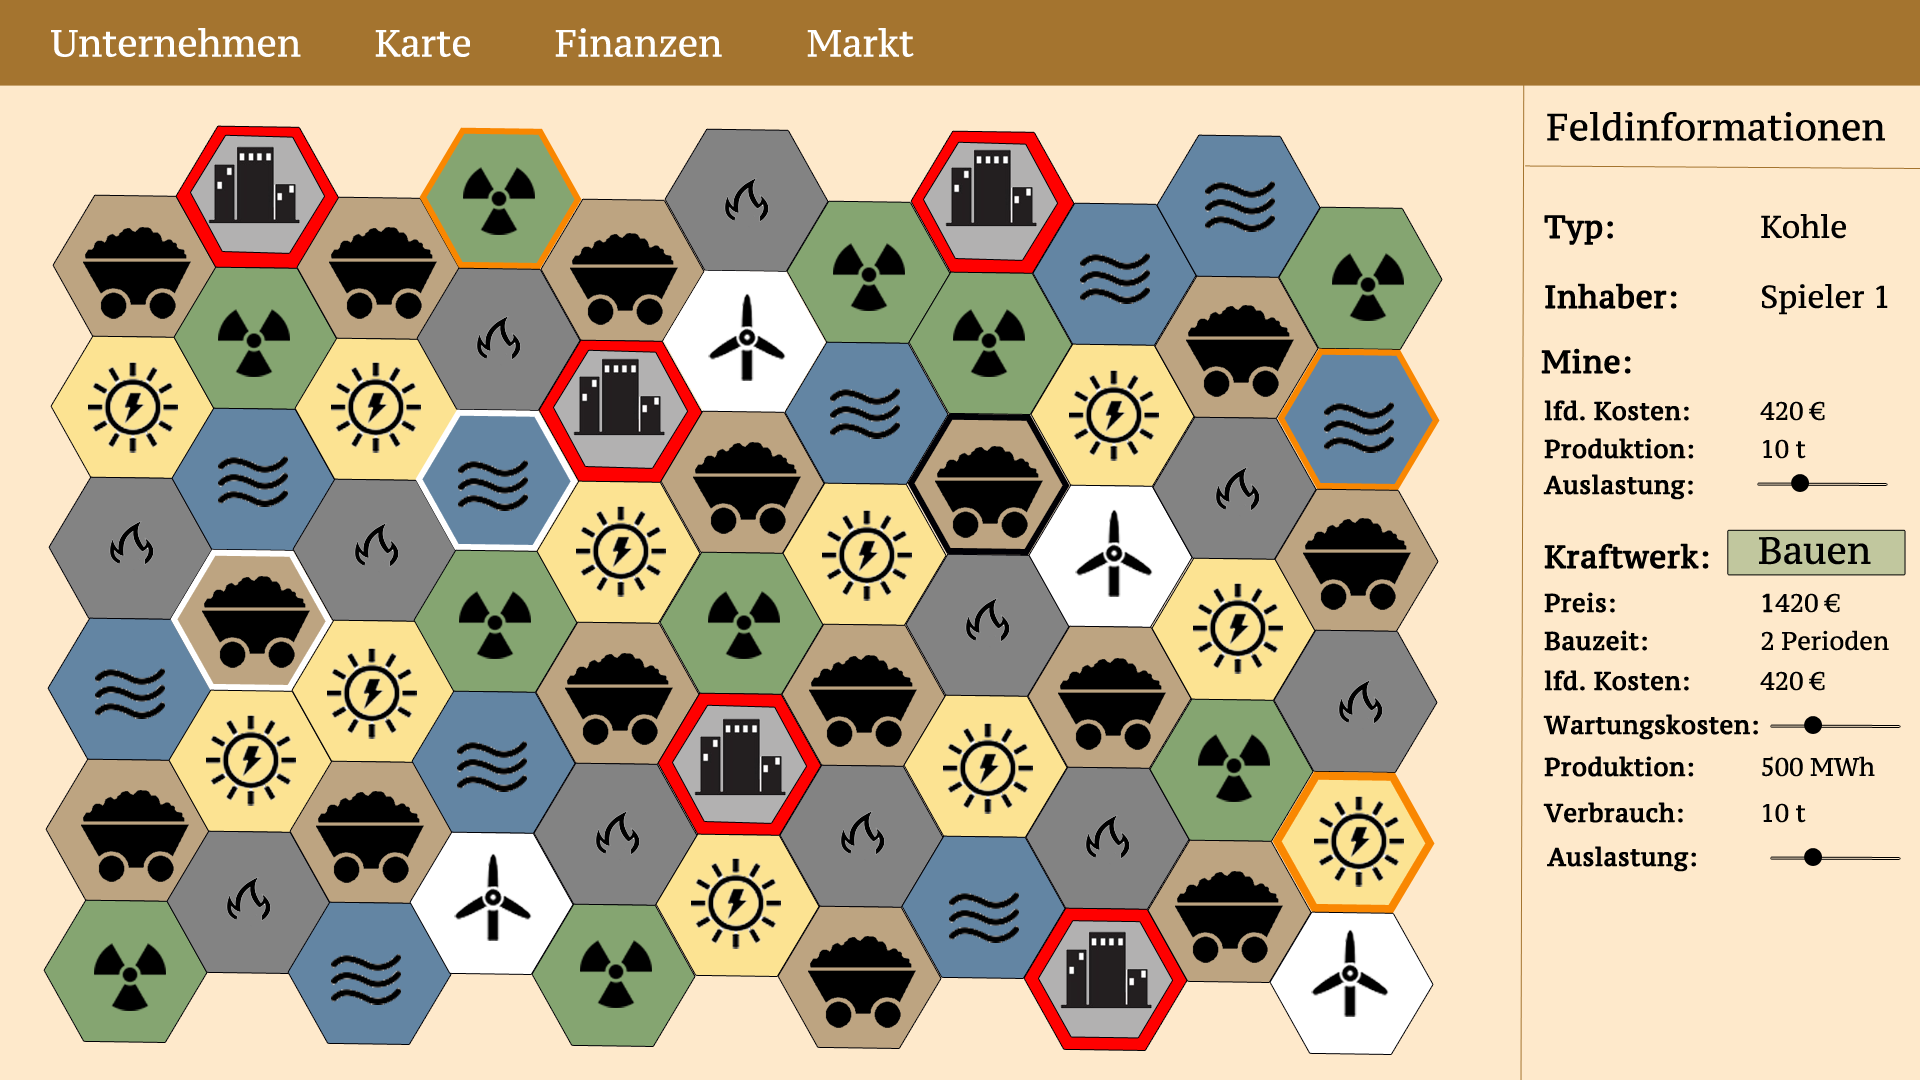
\includegraphics[width=0.8\textwidth]{se-wa-jpg/gui_karte01}
\caption{Karte mit ausgew�hltem Ressourcenfeld}
\label{Karte mit ausgew�hltem Ressourcenfeld}
\end{figure}
Der Typ \textbf{Ressourcen} l�sst sich des Weiteren weiter in folgende Feldern unterteilen:
\begin{itemize}
\item Photovoltaik
\item Kohle
\item Gas
\item Wind
\item Wasser
\item Uran
\end{itemize}

Jeder Typ besitzt dabei eine eigene Farbe und ein eigenes Icon, welche der g�ngigen menschlichen Meinung nachempfunden ist. Dadurch ist es auch m�glich ohne viel Lese- oder Einarbeitungszeit das Spielfeld und die verschiedenen Typen zu verstehen. In den Mockups wurden folgende Farben und Icons gew�hlt:

\begin{table}
    \begin{tabular}{lll}
    \textbf{Typ} & \textbf{Farbe} & \textbf{Icon} \\
    Photovoltaik & gelb & Sonne \\
    Kohle & braun & Kohlewagen \\
    Gas & dunkelgrau & Flamme \\
    Wind & wei� & Windrad \\
    Wasser & blau & Wellen \\
    Uran & gr�n & Atomzeichen\\
    Stadt & hellgrau & Skyline\\
    \end{tabular}
\end{table}

Um nun hervorzuheben, welche Felder sich im Besitz des Spielers oder der Gegenspieler befinden wurde eine farbliche Umrandung des Feldes gew�hlt. Eigene Felder werden dabei in Orange und fremde Felder in wei� umrandet. Eine schwarze Umrandung bedeutet, dass ein Spieler eine Auktion um das Feld er�ffnet hat und darauf geboten werden kann.

Ist ein Ressourcenfeld ausgew�hlt werden in der Sidebar die jeweiligen Feldinformationen angezeigt. Dazu z�hlen sowohl Minen und Kraftwerkinformationen sowie die M�glichkeit diese �berhaupt auch zu bauen, wenn das Feld im Besitz des Spielers ist. Ist es nicht im Besitz des Spielers werden nur wenige Standardinformationen angezeigt.


\subsubsection{Karte mit ausgew�hlter Stadt}
Der Typ \textbf{Stadt} stellt die im Spiel existierenden St�dte dar, welche von
dem Spieler erschlossen werden k�nnen und somit lebensnotwendig f�r jedes
Energieunternehmen sind. Diese Felder sind mit hellgrauer Farbe und
Skyline-Icon gekennzeichnet. Hat der Spieler einen Vertrag zur Belieferung von
Strom mit einer Stadt geschlossen wird diese rot umrandet.

Ist eine Stadt gew�hlt, ist es m�glich �ber die Sidebar Informationen wie z.B. Name und Bev�lkerungsanzahl zu erlangen. Im eigenen Besitz befindende St�dte zeigen ebenso die Anzahl der Kunden als auch die Kosten, Preise, Beliebtheit und Bekanntheit an.

\begin{figure}[H]
\centering
\centering
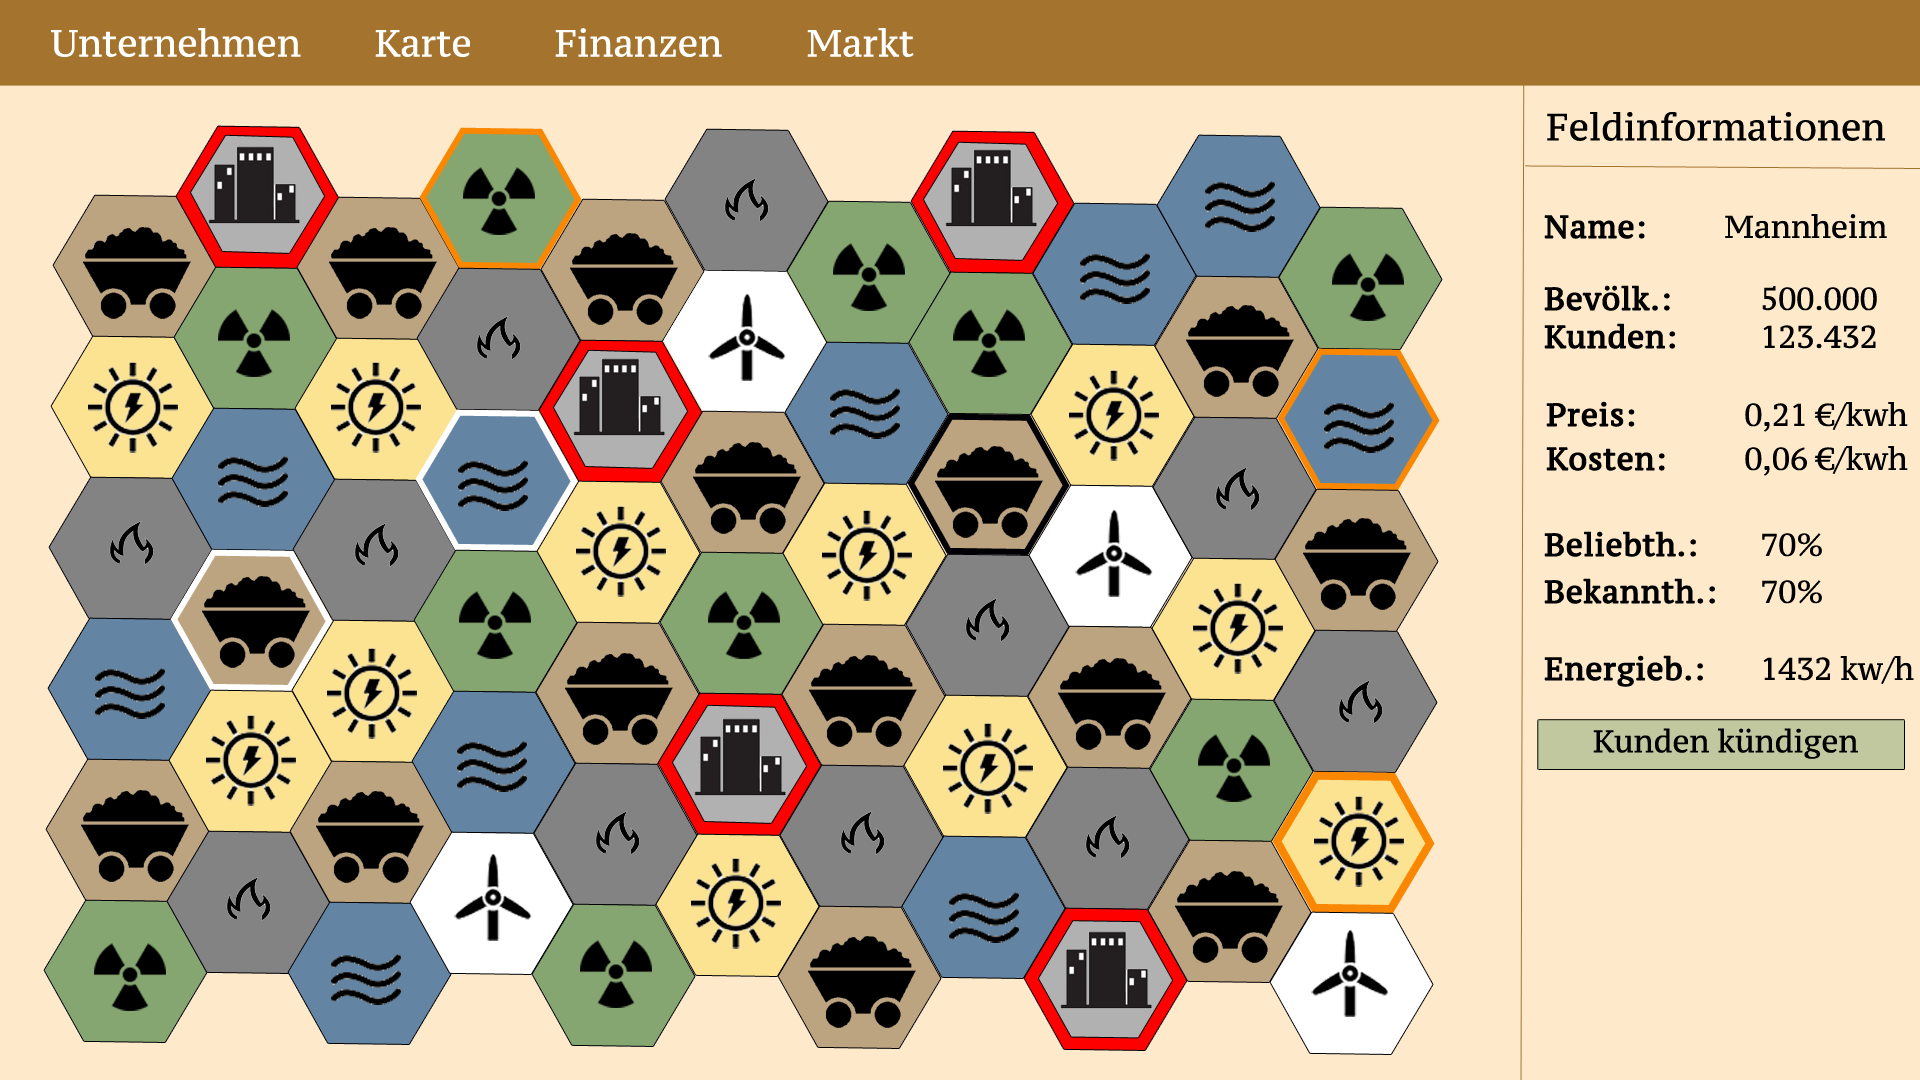
\includegraphics[width=0.8\textwidth]{se-wa-jpg/gui_karte02}
\caption{Karte mit ausgew�hlter Stadt}
\label{Karte mit ausgew�hlter Stadt}
\end{figure}

\subsubsection{Finanzen}
Unter dem Men�punkt ``Finanzen'' ist eine komplette Bilanz sowie Gewinn-- und
Verlustrechnung zu finden. Beide werden in Tabellenform dargestellt und helfen
somit dem Spieler aktuelle Informationen �ber das Unternehmen zu erhalten und
Strategien daraus abzuleiten.
Des Weiteren wird in der Sidebar eine kleine �bersicht �ber die Finanzlage
(Einnahmen und Ausgaben) abgebildet. Sollte es n�tig sein einen Kredit aufnehmen
zu m�ssen, ist dies dort ebenso m�glich sowie die Tilgung der Kredite.

\begin{figure}[H]
\centering
\centering
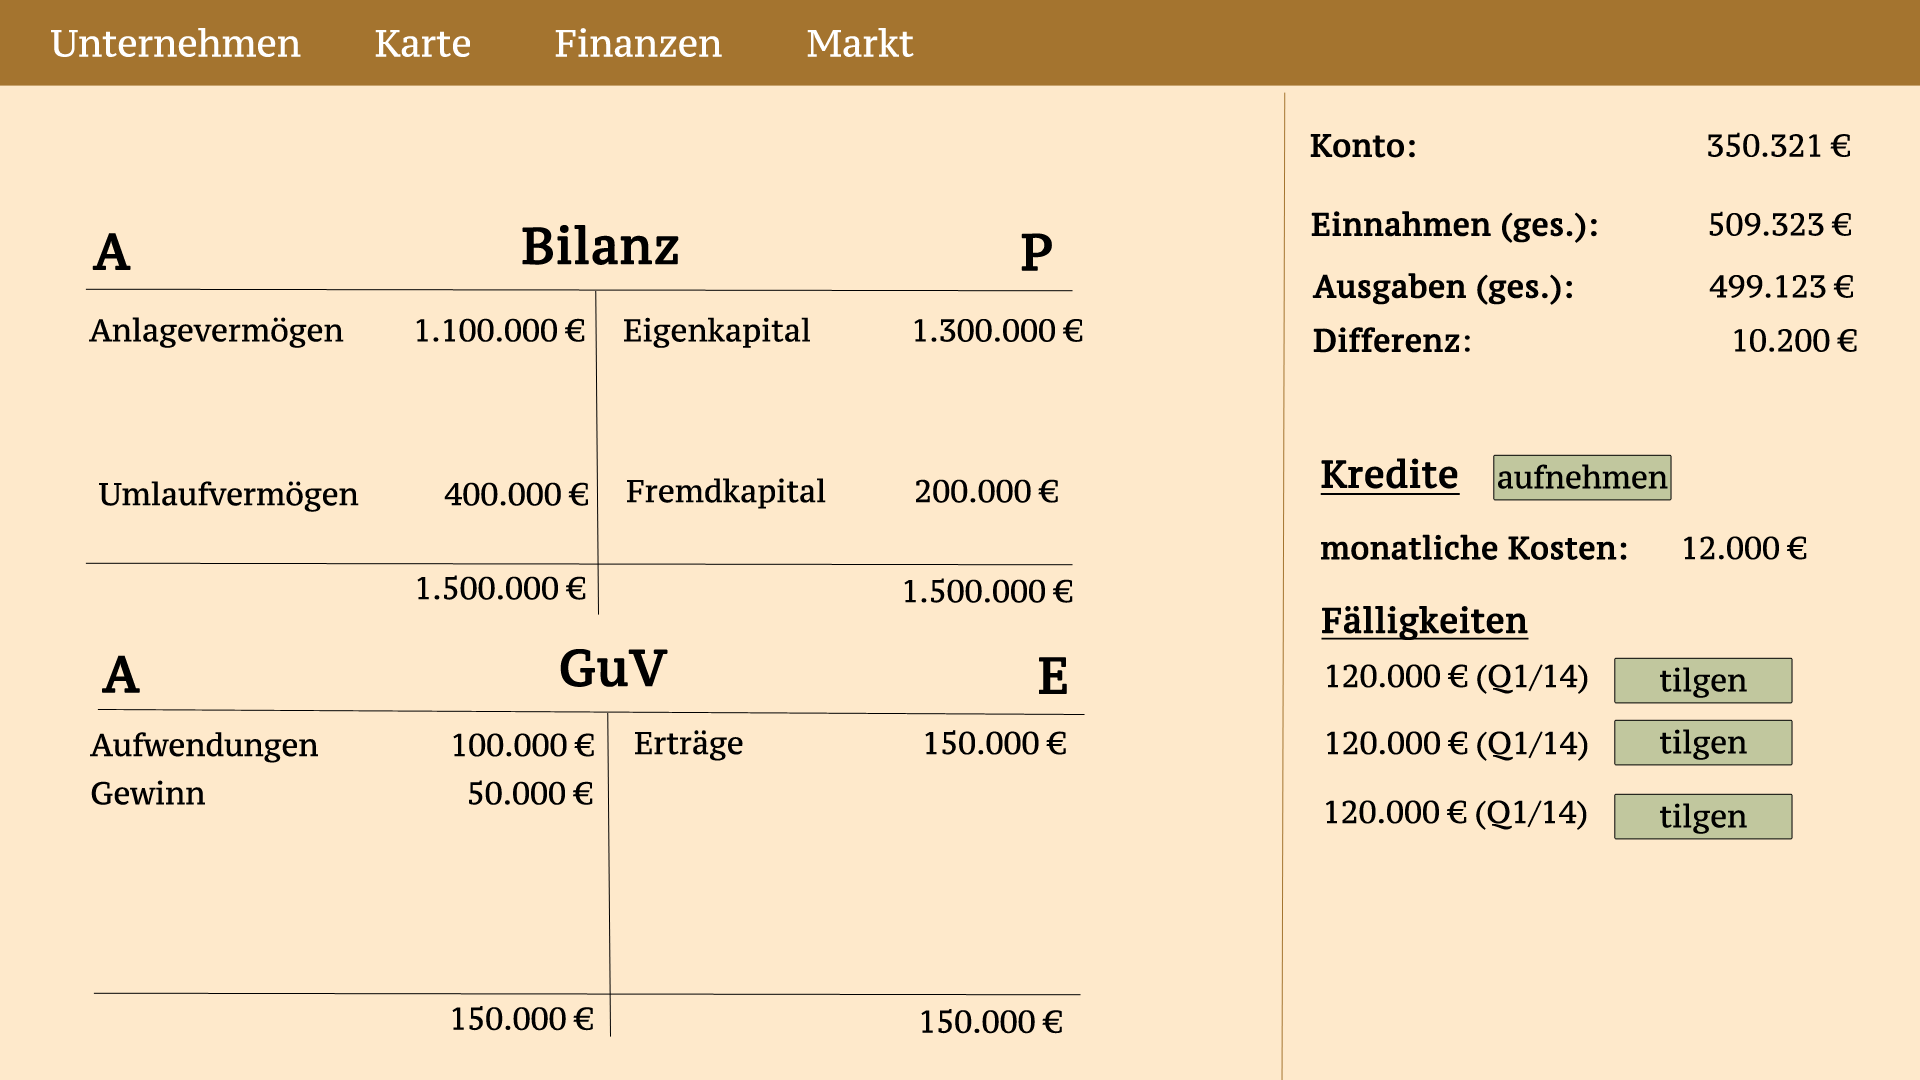
\includegraphics[width=0.8\textwidth]{se-wa-jpg/gui_finanzen}
\caption{Finanzen}
\label{Finanzen}
\end{figure}

\subsubsection{Markt}
Der Markt ist ein Handelsplatz f�r Strom und Rohstoffe. Dort ist es m�glich �ber
Inputfelder Waren zu kaufen und zu verkaufen. Neben den aktuellen Preisen wird ebenso ein Liniendiagramm generiert, welches den Preisverlauf von Strom widerspiegelt und somit eine Art ``Kurs'' abbildet. 
\begin{figure}[H]
\centering
\centering
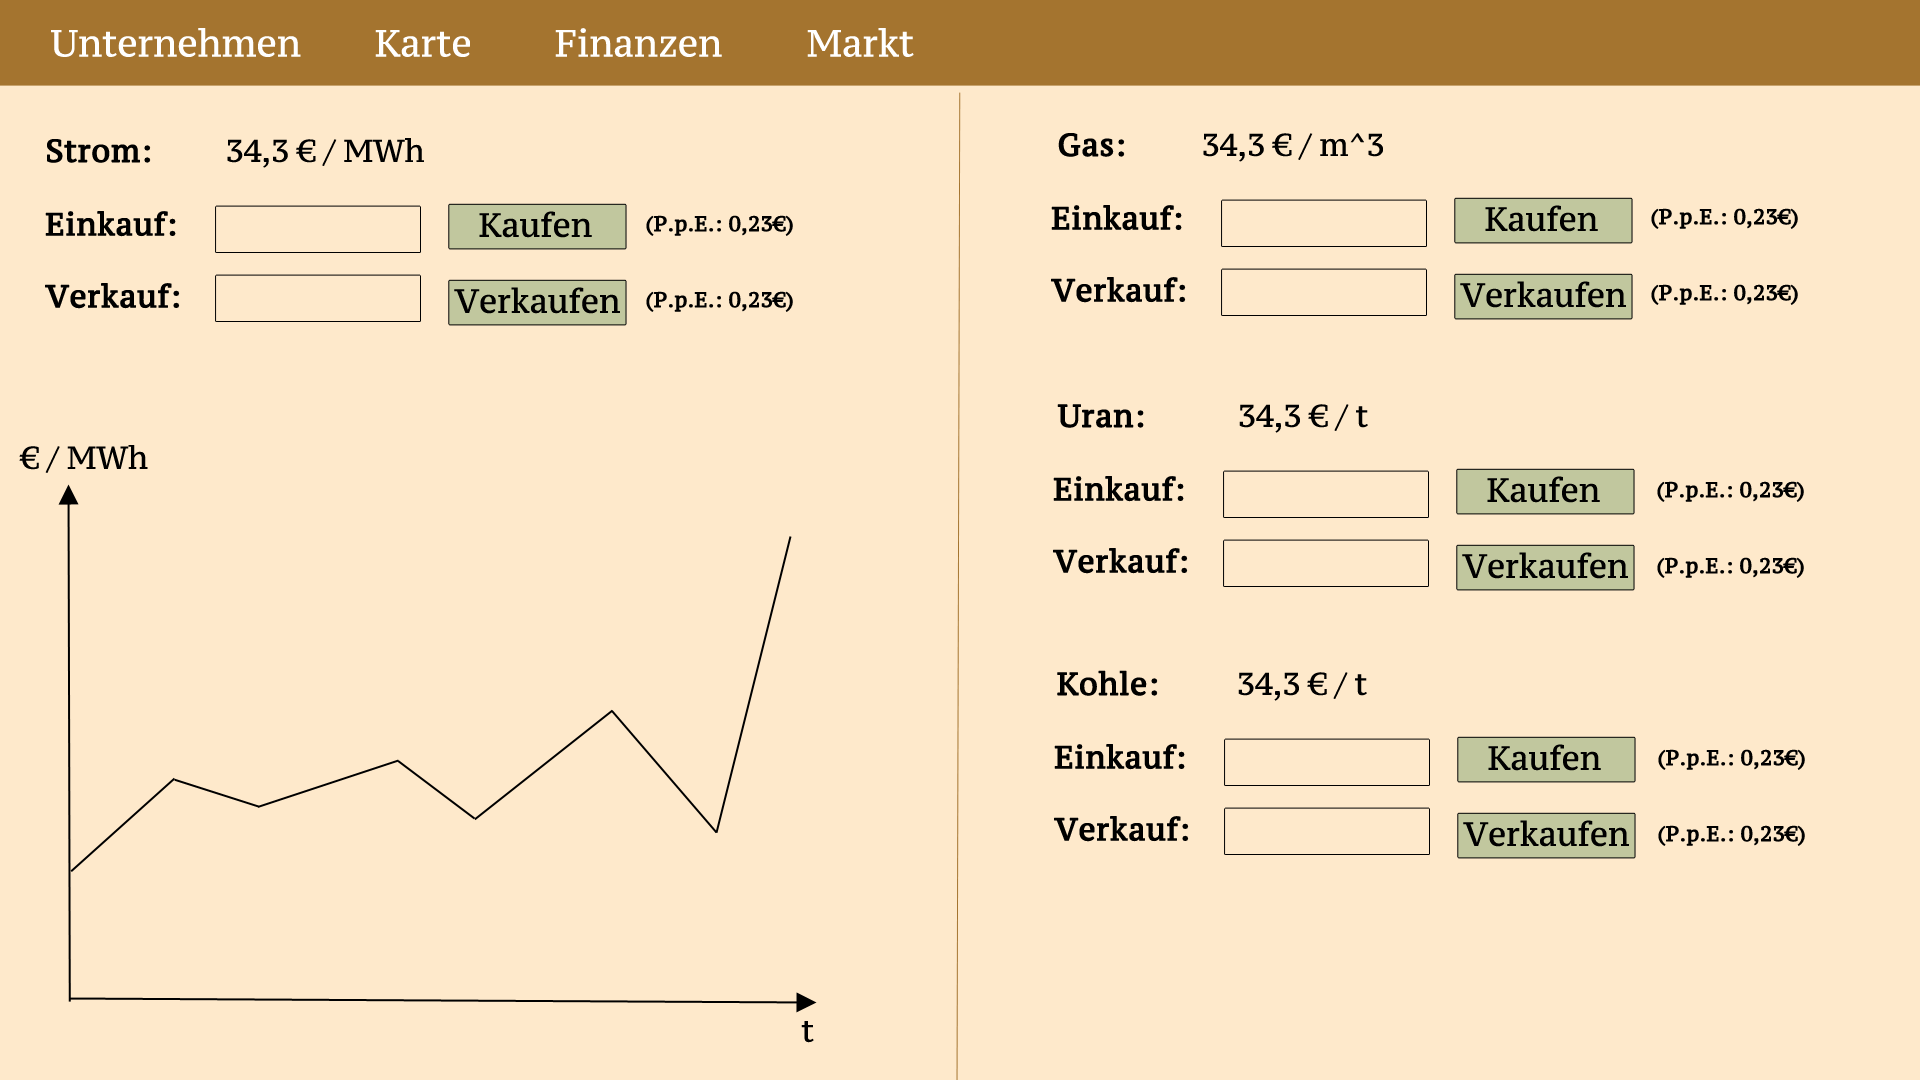
\includegraphics[width=0.8\textwidth]{se-wa-jpg/gui_markt}
\caption{Markt}
\label{Markt}
\end{figure}

\subsection{Ergebnis}
W�hrend der Programmierung wurden etliche Elemente erg�nzt, um das Spiel
angenehmer zu machen und in den Mockups nicht ber�cksichtigte Ereignisse nutzbar zu machen. Im Folgenden werden nur die erg�nzten Elemente der einzelnen Screens genannt und kurz erl�utert.

\subsubsection{Elemente}
Die Anzahl der statischen Elemente hat sich im Vergleich zum Mockup um zwei erh�ht. Dadurch sind folgende Elemente im Planspiel zu finden:
\begin{itemize}
\item Men�leiste
\item Schnell�bersicht
\item Spielerchat
\item Hauptframe
\item Sidebar
\end{itemize}

Die \textbf{Schnell�bersicht} befindet sich rechts neben der Men�leiste und gibt dem Nutzer stets einen �berblick �ber die aktuelle Finanz- und Rohstofflage und informiert den Spieler �ber die Ver�nderungen der Werte, welche in der n�chsten Runde �gebucht� werden. Somit ist kein l�stiges Wechseln des Men�punktes n�tig, um diese Informationen zu erhalten. 

Der \textbf{Spielerchat} ist ein kleines Zusatzfeature, welches am linken Rand zu lokalisieren ist. Mit diesem ist es m�glich mit seinen Mit- bzw. Gegenspielern zu kommunizieren. Der Chatverlauf kann von allen Teilnehmern eingesehen werden.


\subsubsection{Startscreen}
Nachdem der Spieler das Spiel gestartet hat landet dieser auf dem Startbildschirm. Dieser erscheint in einem modernen Popup-Look. Dort muss die IP-Adresse, der Spielername und der Firmenname eingetragen werden, um das Spiel zu starten. Der Startscreen sowie der folgende Lobby-Bildschirm wurden in keinem Mockup veranschaulicht oder vorher gro� geplant, wodurch kein Vergleich m�glich ist.

\begin{figure}[H]
\centering
\centering
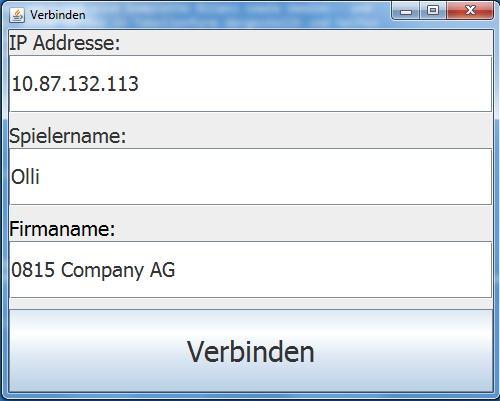
\includegraphics[width=0.8\textwidth]{se-wa-jpg/gui_start}
\caption{Startscreen}
\label{Startscreen}
\end{figure}

\subsubsection{Lobby}
Auf den Startbildschirm folgend wird der Spieler in die Lobby weitergeleitet, in
der es m�glich ist auf weitere Mitspieler zu warten, um z.B. gegen Freunde zu
spielen. Klickt der Spieler auf �Bereit� startet das Spiel sobald alle anderen Mitspieler ebenso diese Aktion ausgef�hrt haben.
\begin{figure}[H]
\centering
\centering
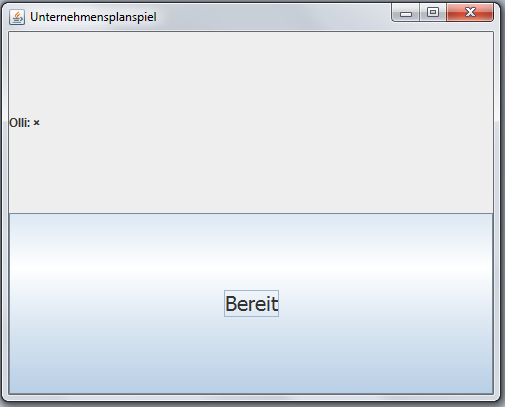
\includegraphics[width=0.8\textwidth]{se-wa-jpg/gui_login}
\caption{Lobby}
\label{Lobby}
\end{figure}

\subsubsection{Unternehmen}
Die Unternehmens�bersicht hat sich im Vergleich zum Mockup nicht ge�ndert.

\begin{figure}[H]
\centering
\centering
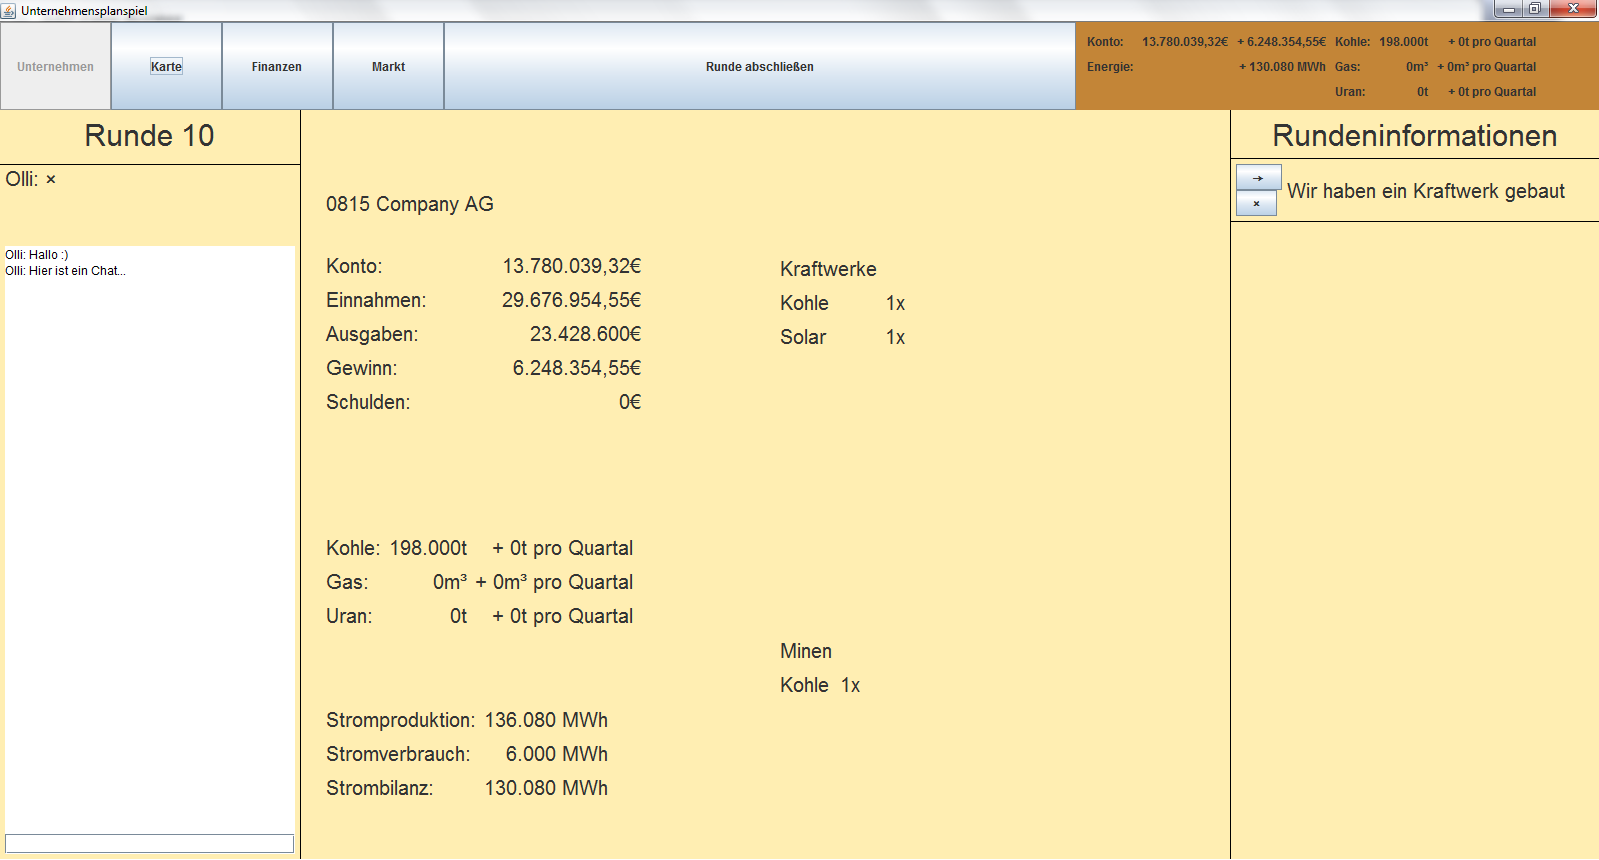
\includegraphics[width=0.8\textwidth]{se-wa-jpg/gui_result_unternehmen}
\caption{Unternehmen}
\label{Unternehmen}
\end{figure}

\subsubsection{Karte mit ausgew�hltem Ressourcenfeld}
Der Grundaufbau der Karte hat sich im Vergleich zum Mockup nur leicht ge�ndert. So wurde die Form des Spielfeldes der einzelnen Felder angepasst und ist ebenso wie ein Hexagon geformt. 

Au�erdem wurden einige Icons und Farben von Feldern angepasst, um farblich besser hervorzustechen. Das Ergebnis sieht folgende Farben und Icons vor:

\begin{table}
    \begin{tabular}{lll}
    Typ & Farbe & Icon \\
    Photovoltaik & gr�n & Solarpanel \\
    Kohle & braun & Kohlewagen \\
    Gas & dunkelgrau & Flamme \\
    Wind & hellgrau & Windrad \\
    Wasser & blau & Wassertropfen \\
    Uran & gelb & Atomzeichen\\
    Stadt & lila & Skyline\\
    \end{tabular}
\end{table}

Neben diesen �nderungen hat man auch die Umrandungen von betroffenen Feldern angepasst und neue hinzugef�gt:

\begin{table}
    \begin{tabular}{lll}
    Farbe & Beschreibung \\
    rosa & Felder, die im Besitz des Spielers sind \\
    turkis & Felder, bei denen eine Auktion durch einen beliebigen Spieler gestartet wurde \\
    schwarz & Ressourcenfeld, auf dem eine Mine gebaut wurde
    \end{tabular}
\end{table}

Eine besonders hilfreiche Funktion ist auch die automatische Zuordnung der Energiequellen zu den Verbraucherst�tten. Damit wird eine Verkn�pfung zwischen Feldern hergestellt, die sich gegenseitig Energie liefern. Die sogenannte Verkn�pfungslinie ist rot.

An der Sidebar wurden keine �nderungen vorgenommen.

\begin{figure}[H]
\centering
\centering
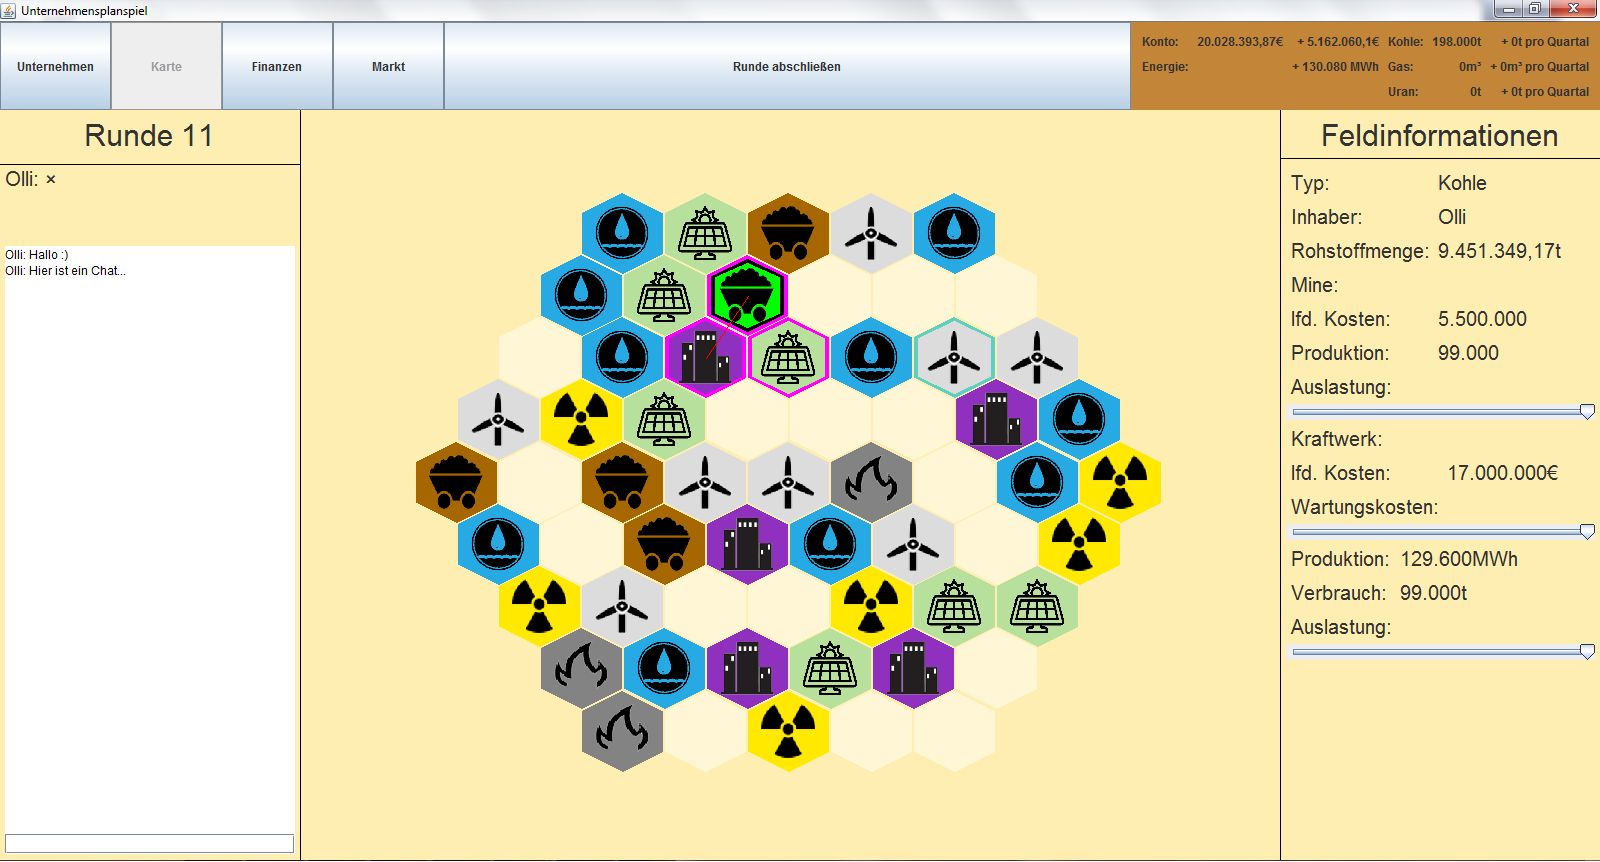
\includegraphics[width=0.8\textwidth]{se-wa-jpg/gui_karte_ressource}
\caption{Karte mit ausgew�hltem Ressourcenfeld}
\label{Karte mit ausgew�hltem Ressourcenfeld}
\end{figure}




\subsubsection{Karte mit ausgew�hlter Stadt}
Bei dieser Ansicht wurden die Sidebarinformationen nach den Spielbed�rfnissen angepasst und formatiert. Ansonsten hat es keine Ver�nderungen zu Mockup gegeben.

\begin{figure}[H]
\centering
\centering
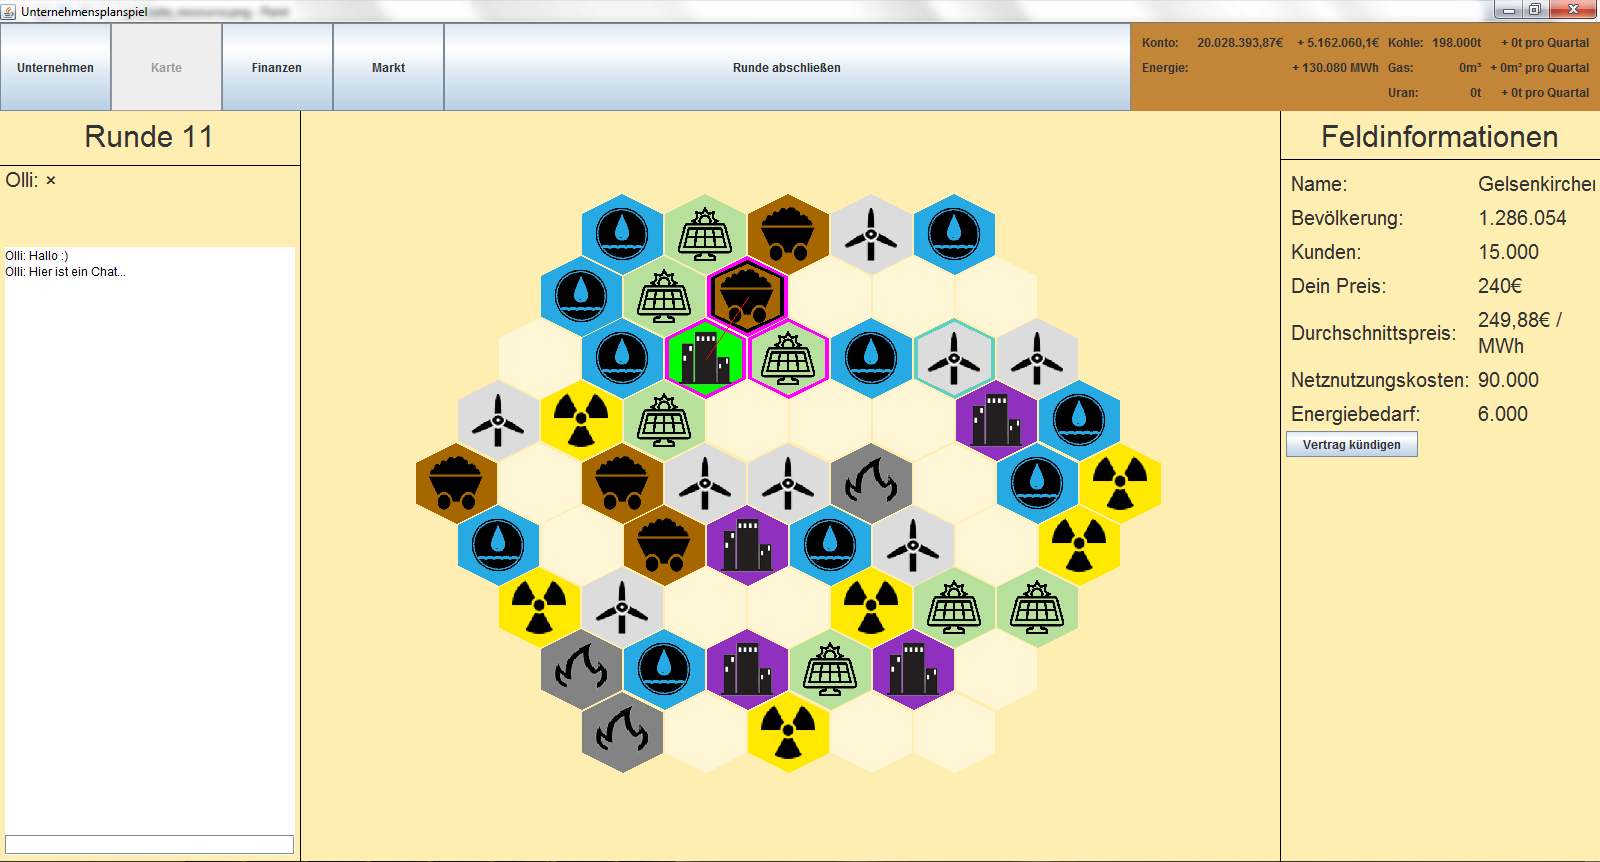
\includegraphics[width=0.8\textwidth]{se-wa-jpg/gui_karte_city}
\caption{Karte mit ausgew�hlter Stadt}
\label{Karte mit ausgew�hlter Stadt}
\end{figure}

\subsubsection{Finanzen}
Die Finanzen werden in unserer Endfassung sehr detailliert dargestellt. So sind in der Bilanz und der Gewinn- \& Verlustrechnung alle n�tigen Posten gelistet. Die in unserem Mockup gelistete Funktion �Kredit tilgen� wurde jedoch entfernt, sodass es nun nur m�glich ist einen Kredit aufzunehmen. Des Weiteren sind nun direkt die Kreditkonditionen zusehen, was die Aufnahme deutlich vereinfacht.
\begin{figure}[H]
\centering
\centering
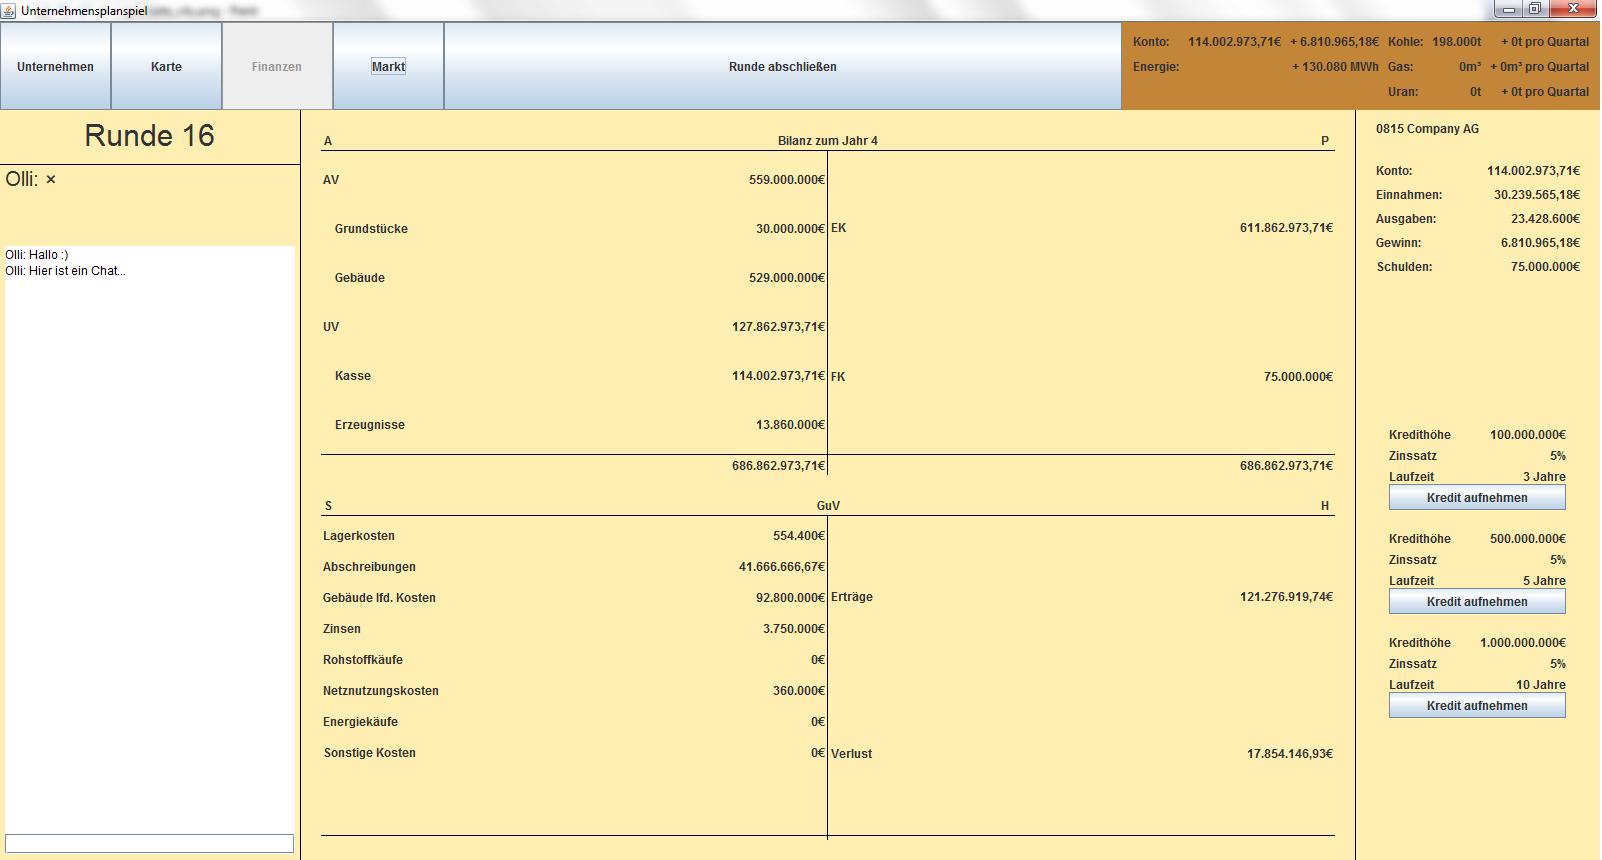
\includegraphics[width=0.8\textwidth]{se-wa-jpg/gui_result_finanzen}
\caption{Finanzen}
\label{Finanzen}
\end{figure}

\subsubsection{Markt}
Auf Grund des hohen Entwicklungsaufwandes wurde das vorgesehen Diagramm weggelassen. Dieses sollte den Verlauf des Strompreises darlegen.
\begin{figure}[H]
\centering
\centering
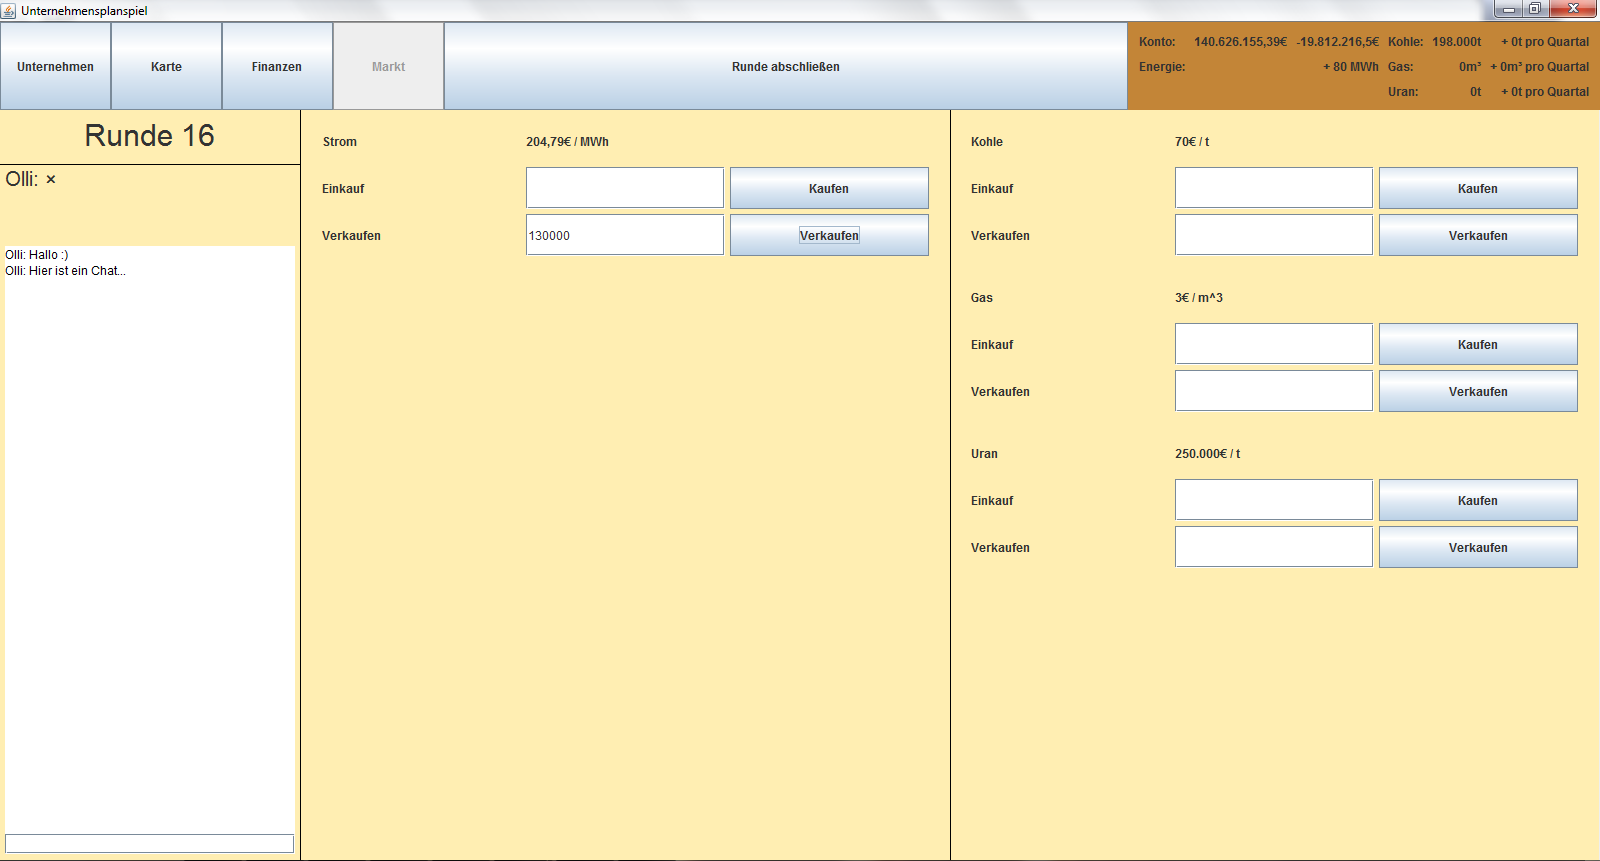
\includegraphics[width=0.8\textwidth]{se-wa-jpg/gui_result_markt}
\caption{Markt}
\label{Markt}
\end{figure}

\subsection{Fazit}
Im Gro�en und Ganzen wurde ein guter Entwicklungsprozess durchgezogen. So wurden St�ck f�r St�ck Verbesserungen vorgenommen und somit das Spiel komplettiert. Von der Skizze �ber das Mockup bis hin zum Endergebnis wurden viele Varianten ausprobiert und im Team diskutiert. Dadurch konnte ein Ergebnis erzielt werden, welches alle Teammitglieder zufriedenstellt. Durch einige Verbesserungen k�nnte das Spiel eine noch bessere Oberfl�che bekommen. Unser Hauptaugenmerk lag jedoch in der Programmierung und nicht im Design einer grafischen Oberfl�che.

\subsection{Verbesserungsm�glichkeiten}
Trotz der bereits vielen Optimierungen sind weitere Verbesserungen m�glich:
\begin{itemize}
\item Gr��enanpassung der Icons in der Karte
\item Optimierung der Farben (mehr Komplement�rfarben)
\item Einbindung von Diagrammen
\item teilweise bessere Formatierung von Texten und Werten
\end{itemize}
%Olli
\section{Graphische Benutzeroberfl�che}\label{olli:gui}
In dieser Sektion wird der Aufbau der graphischen Benutzeroberfl�che (GUI)
erl�utert, die mit Java Swing entwickelt wurde. Zun�chst wird das GUI durch die
Singleton Klasse \textbf{Controller} verwaltet und durch diese wird
sichergestellt, dass von dem GUI die aktuellen Informationen angezeigt werden.
Des Weiteren bietet es den GUI Klassen den Zugriff auf das Datenmodell. Die GUI
Klassen liegen im Paket \textbf{de.client.gui}. 
%In der �berwiegenden Mehrheit
%sind einzelne Komponenten durch lazy initialization

\subsection{Globale Bestandteile}
Allgemein werden die ben�tigten JPanels immer in ein Objekt der Klasse
\textbf{Frame} eingef�gt --- dies ist das Fenster, das f�r das Spiel verwendet
wird.
\begin{itemize}
  \item Ein \textbf{PanelGlobalLeft} befindet sich immer auf der linken Seite
  des Fensters, in dem die Liste von Spielern mit ihrem Status und der Chat 
  enthalten sind. Diese beiden Einzelteile werden von dem Controller
  aktualisiert, wenn der Client eine Nachricht vom Typ  
  \texttt{PLAYER\_READY\_CHANGE} bzw. \texttt{CHAT\_BROADCAST} erh�lt.
  \item Das Men� wird durch ein \textbf{PanelMenu} dargestellt, das die Buttons
  und ein \textbf{PanelMenuInformation} enth�lt. \textbf{PanelMenuInformation}
  besteht aus einem JLabel mit einem Text, der HTML Code enth�lt --- dadurch
  entsteht die Tabellenstruktur. 
  \item \textbf{PanelAbstractContent} wird bei allen Tabs au�er dem Markt
  verwendet: In dieser abstrakten Klasse werden zwei JPanels definiert, dessen
  Layout mithilfe eines \textbf{GridBagLayout} in der Methode
  \textbf{initLayout()} festgelegt wird. Durch die Festlegung eines linken und
  eines rechten Panels soll ein einheitliches Layout in allen Tabs entstehen ---
  des Weiteren wird hier bereits die Hintergrundfarbe und die R�nder gesetzt.
\end{itemize}

Wichtig ist au�erdem die Klasse \textbf{Look}, in dem statisch die verschiedenen
Hintergrundfarben und die R�nder der hexagonf�rmigen Buttons in der Karte
definiert sind. Des Weiteren wurde die Klasse \textbf{Strings} erstellt, die
mehrere statische Methoden bereit stellt, die Daten f�r die Anzeige im GUI vorbereiten
soll --- darunter zum Beispiel die Funktion \textbf{fD(double number)}, die
Zahlen, besonders vom Typ \textbf{double}, lesbarer machen soll. Au�erdem
besitzt sie Attribute wie \textbf{ENERGY\_UNIT}, damit diese an einer Stelle
definiert sind und auch einheitlich ver�ndert werden k�nnen.

Nach dem Mockup wurden vier unterschiedliche Tabs entwickelt, die dem Spieler
unterschiedliche Einblicke in sein Unternehmen geben sollen:

\subsection{Unternehmensplanung}
Die Unternehmensplanung ist �hnlich wie die meisten anderen Tabs aus zwei
Panels aufgebaut und wird durch ein \textbf{PanelCompany} dargestellt, das von 
\textbf{PanelAbstractContent} erbt. 

Das linke (im Fenster mittlere) Panel ist ein \textbf{GridLayout} mit zwei
Spalten und zwei Reihen und wird von JLabels gef�llt. Die Tabellenstruktur in
den einzelnen JLabels entsteht �hnlich wie im Men� durch die Nutzung von HTML 
Code. Die rechte Seite enth�lt die Nachrichten, die dem Spieler zum Beginn der 
Runde angezeigt werden.

\subsection{Karte}\label{GUIKarte}
Die Karte ist das Herzst�ck der Benutzeroberfl�che --- hier kann der Spieler die
wichtigsten Entscheidungen wie das Bauen von Kraftwerken und das Schlie�en von
Vertr�gen treffen. Insgesamt ist der Kartentab ein \textbf{PanelMain}, das
ebenfalls von \textbf{PanelAbstractContent} erbt. Zun�chst wird die linke (im
Fenster mittlere) Seite erkl�rt.

Das \textbf{PanelMap} selbst enth�lt nur viele \textbf{HexagonButton}, dessen
Positionen von einem \textbf{HexagonLayout} verwaltet werden. Die Implementation
des HexagonLayout wurde anfangs von (\seCite{}{}{codeguru})  �bernommen. Dieses
besa� am Anfang nur ein rechteckiges Layout --- es wurde anschlie�end angepasst,
damit beispielsweise die H�he und Breite der Buttons korrekt bei �nderung der 
Fenstergr��e mitskaliert werden. Des Weiteren wurde ein hexagonf�rmiges Layout 
implementiert, das unserer Spielidee n�her liegt: Das GUI kann beide 
Kartenarten darstellen.

Jeder \textbf{HexagonButton} erh�lt bei der Initialisierung eine
\textbf{Region}, mit der er seine Hintergrundfarbe, R�nder und das Bild
bestimmten kann. Des Weiteren besitzt er eine Referenz zu einem
\textbf{PanelSubDetails}: Diese wird bei dem ersten Klick auf dem Button
initialisiert und bleibt danach erhalten. Der Inhalt davon wird durch einen
Entscheidungsbaum in \textbf{PanelDetails.setRegionContent} bestimmt.

Durch ``Lazy Initialization'' des \textbf{PanelSubDetails} wird hier auf lange
Sicht Rechenzeit gespart, daf�r wird jedoch mehr Speicherplatz ben�tigt. Das
\textbf{PanelSubDetails} wird dann jeweils in die rechte Seite des
Kartentabs, die durch ein \textbf{PanelDetails} dargestellt wird, eingef�gt.

Erh�lt der Client durch eine \textbf{MAP\_UPDATE} Nachricht ist die Runde
beendet: Die Referenz zum alten \textbf{PanelMap} wird gel�scht und ein komplett
neues Objekt wird angelegt --- deswegen flackert das GUI kurz, sobald eine Runde
beendet ist.

\subsection{Finanzen}
Die finanziellen Informationen der Firma werden durch ein \textbf{PanelFinances}
abgebildet: Auf der linken Seite befindet sich ein
\textbf{PanelFinancesBalance}, das durch viele verschachtelte 
\textbf{GridLayout} konstruiert wird. Hier wird die Bilanz und die GuV des
Unternehmens dargestellt.Daneben besteht die rechte Seite aus
einem JLabel mit HTML Code und einem \textbf{PanelCredits}, in dem
Informationen zu den verschiedenen Kredittypen angezeigt werden.

\subsection{Markt}
Die beiden Seiten des Marktes sind relativ gleich aufgebaut und befinden sich in
einem \textbf{PanelMarket}. Sie besitzen beide ein \textbf{BoxLayout}, damit
Komponenten vertikal untereinander eingef�gt werden. Die Anzeige der einzelnen
Rohstoffe, die hier gekauft und verkauft werden k�nnen, werden durch ein
\textbf{PanelMarketResource} erstellt und basieren auf der Enumeration
\textbf{de.shared.map.region.BuyableResouce}.
%Olli
\newpage
\section{Unit Tests}
In diesem Projekt wurde versucht, m�glichst fl�chendeckend und detailiert Unit
Tests zu erstellen. Deswegen haben wir uns f�r zwei Kategorien von Unit Tests
entschieden: Erstens die, die die Spielelogik testen sollen und zweitens
Szenariotests, die ganze Spielemechaniken und die Kommunikation zwischen
Client und Server testen sollen.

Damit wurde nach dem Eclipse Plugin ``EclEmma'' insgesamt ein Code Coverage von
ca. 80\% erreicht (ohne Betrachtung des Codes in \texttt{de.tests} und des Codes in
\texttt{de.client.gui}, der die graphische Benutzeroberfl�che generiert).

\subsection{Spielelogik}
Unter diese Kategorie fallen alle Tests, die Funktionalit�ten des Spieles ohne
Client Server Kommunikation testen.

\begin{itemize}
  \item \texttt{de.tests.client}: In diesem Paket sind zwei Tests
  enthalten, die die finanziellen Aspekte des Spieles testen soll --- dazu
  geh�ren die folgenden Tests: \texttt{TestInvestmentDepreciation}, der die
  Abschreibung von Grundst�cken und Geb�uden testet und \texttt{TestWarehouse},
  in dem die Verwaltung von Rohstoffen getestet wird. 
  \item \texttt{de.tests.client.optimization}: Hier wird die Optimierung der
  Kraftwerke getestet. Dazu gibt es eine Hilfsklasse \texttt{TestObjectFactory}, die f�r
  die vier Tests die erforderlichen Objekte statisch erzeugt. 
  \item \texttt{de.tests.client.gui}: Tests in diesem Paket sind keine Unit
  Tests im eigentlichen Sinne eines automatischen Durchganges sondern wurden erstellt, um
  das Testen der graphischen Benutzeroberfl�che zu erleichtern. F�r jeden Tab
  der Benutzeroberfl�che gibt es eine Klasse.
  \item \texttt{de.tests.shared.map}: In dem letzten Paket wird durch
  \texttt{GenerateRegions} getestet, ob die Regionen richtig erzeugt werden und
  in \texttt{TestEnergyExchange} werden die Funktionalit�ten der Energieb�rse
  getstet. 
\end{itemize}

\subsection{Szenariotests}
Die zweite Kategorie von Unit Tests sind die Tests in
\texttt{de.tests.clientserver}, die die Kommunikation zwischen den Clients und
dem Server testen. Dabei ist zun�chst wichtig, dass die Klasse \texttt{Server}
das Singleton Pattern implementiert und deswegen zwischen den einzelnen Tests
mit der Methode \texttt{reset} zur�ckgesetzt werden muss --- hier wird das
\texttt{ServerSocket} geschlossen und wieder neu er�ffnet.

Des Weiteren erbt jeder Test in diesem Paket von
\texttt{AbstractClientServerTest}, der \texttt{@Before} und \texttt{@After}
Methoden definiert, damit der Server zwischen den Tests neugestartet wird.

Bei einem JUnit Test werden alle Methoden, die als \texttt{@Test} markiert sind,
als neue Thread gestartet und parallel ausgef�hrt. Da dies bei gleichzeitigen
Client Server Tests zu Schwierigkeiten wegen des \texttt{ServerSocket}  f�hren
w�rde, wurde die Klasse \texttt{ClientServerMonitor} konzipiert. Diese
implementiert aus zwei Gr�nden das Singleton Pattern: Erstens muss ein Monitor 
f�r die \texttt{Object.wait()} Methode objektorientiert und nicht statisch sein
und zweitens um eine Referenz bei jeder Testklasse zu sparen. Die Methode 
\texttt{startTest()} wird vor dem Start eines Tests aufgerufen --- damit werden
alle anderen Threads, die auch dieses Methode aufrufen, durch
Warten ausgeschlossen. Ist ein Test beendet wird die \texttt{endTest()} Methode
aufgerufen, die dann alle anderen Test Threads wieder aufweckt. 

In der \texttt{@Before} Methode der \texttt{AbstractClientServerTest} Klasse
wird also \texttt{startTest()} und in der \texttt{@After} Methode
\texttt{endTest()} aufgerufen.




















%Patrick
\section{BWL und Balancing}\label{patrick:balancing}
\subsection{Umsetzung betriebswirtschaftlicher Besonderheiten}
Die Besonderheiten, die wir bei der Analyse der betriebswirtschaftlichen
Grundlagen erarbeitet haben, wurden in unserem Planspiel verwirklicht, in dem
die Stromproduktion verschiedener Kraftwerke unterschiedlich geregelt werden kann.

Der Betrieb von Kern- und Kohlekraftwerken wiederum sorgt f�r Unzufriedenheit in
der Bev�lkerung und senkt somit die Beliebtheit des Betreibers. Diese
Funktionalit�t wurde auch in das Spiel integriert und hat Auswirkungen auf die
Zahl der Vertr�ge, die in einer Stadt abgeschlossen werden.
Die Stadt ist neben den ``Baufeldern'' das zentrale Medium um einen finanziellen
Umsatz in dem Spiel zu generieren. Durch das Anbieten einer verf�gbaren
Kapazit�t zu einem festgelegten Preis, wird ein Vertrag mit der Stadt und somit
einer gewissen Anzahl an Kunden erstellt. Je nach Anbietern bei dieser Stadt und
je nach vorgeschlagenem Preis, hat das Unternehmen eine gewisse Anzahl an
Kunden.

Die weitere M�glichkeit, �ber die im Planspiel Geld verdient werden kann ist,
den Strom �ber die Stromb�rse zu verkaufen. Allerdings ist diese so
programmiert, dass sie sich auch wie an einer ``echten'' B�rse verh�lt, das hei�t
je mehr Angebot vorhanden ist desto geringer ist der Preis.
Eine dritte M�glichkeit Geld zu verdienen, welche allerdings der Spielidee
entgegensteht, ist es, nach dem Bau von Minen die dort produzierten Rohstoffe an
dem Markt zu verkaufen.

\subsection{Festlegung betriebswirtschaftlicher Werte im Planspiel}
Im Folgenden ist eine Kosten�bersicht, die neben den laufenden Kosten und den
Baukosten auch die Bauzeit und die Leistung der einzelnen Kraftwerke beinhaltet.

<TABELLE 1>

Die obige Tabelle zeigt die im Spiel implementierten, von Anfang an festgelegten
Daten. Dabei handelt sich um eine reine �bersicht der Baukosten und -zeit und
die laufenden Kosten. Ein Kernkraftwerk kostet 3,1 Milliarden Euro und es dauert
10 Quartale, eins zu bauen. Damit ist dies das teuerste Kraftwerk in der
Anschaffung, allerdings sind die laufenden Kosten nicht so hoch und durch den
gro�en Leistungsunterschied zu den anderen Kraftwerken ist es m�glich, einen
hohen Gewinn erreichen. 
Im Gegensatz dazu kann eine Photovoltaikanlage innerhalb von einem Quartal
gebaut werden und kostet 45 Millionen Euro, wodurch dies das g�nstigste
Kraftwerk in der Anschaffung ist. Allerdings betr�gt die Leistung nur ein
Bruchteil (genauer: ein f�nfzigstel?) von dem Kernkraftwerk.

Alle Werte wurden so festgelegt, dass die Bauzeit, die Leistung, die Baukosten
sowie die laufenden Kosten in Relation zueinander stehen.
(Willst du hier nicht wenigstens jedes Kraftwerk mal kurz konkret erw�hnen mit seinen Daten?)

Abgesehen vom Bau der Kraftwerke besteht auch noch die M�glichkeit, auf den
Kohle-, Gas- und Kernkraftwerkfeldern Minen zu bauen. Diese Felder produzieren
Kohle, Gas beziehungsweise Uran. (wof�r brauch ich das?)

<Tabelle 2>

Auch die Minen m�ssen erst gebaut werden, was eine gewisse Zeit in Anspruch
nimmt und wobei auch Kosten entstehen. Hierbei ist zum Beispiel ein Augenmerk
auf die Gas-Mine zu legen, da hier die Bauzeit l�nger ist, als der eigentliche 
Bau eines Kraftwerks. Somit muss entweder erst die Mine gebaut werden, bevor das
Kraftwerk in Auftrag gegeben wird oder die ben�tigten Rohstoffe werden f�r die
ersten zwei Quartale von dem Rohstoffmarkt bezogen. Durch den Abbau der
jeweiligen Rohstoffe sind auch bei einer Mine laufende Kosten zu entrichten.

Die letzten beiden Spalten der Grafik beschreiben sowohl die Menge an
Rohstoffen, die ein Kraftwerk pro Quartal ben�tigt, als auch die Kosten f�r den
Bezug der Rohstoffe vom Rohstoffmarkt. Diese Kosten sind nicht variabel sondern
bleiben stetig gleich.

Die Festlegung des Startkapitals erfolgte erst nach der Bestimmung aller anderen
Werte, da erst danach ein sinnvoller Startwert, aufbauend auf diesen Werten,
ermittelt werden konnte. Der Wert von 650 Millionen Euro war das Ergebnis
unserer Ermittlungen. Mit diesem Startkapital kann sowohl die zweitgr��te
Kraftwerksart gebaut werden, als auch einige kleinere, sodass jeder Spieler die
M�glichkeit hat, sich je nach Interesse im Markt auszurichten.

Falls ein Spieler eine gr��ere Investition t�tigen m�chte oder Probleme mit
liquiden Mitteln hat, besteht die M�glichkeit Kredite aufzunehmen. Diese sind in
drei unterschiedliche Kreditgr��en aufgegliedert:

\begin{itemize}
  \item 100 Millionen
  \item 500 Millionen
  \item 1 Milliarde
\end{itemize}

Dem Spieler steht die M�glichkeit zur Verf�gung so viele Kredite aufzunehmen wie
er m�chte, allerdings darf die gesamte Kreditsumme dabei nicht mehr als das
Zweifache des Eigenkapitals betragen.
Die Kredite sind allesamt mit einem Prozentsatz von 5 \% verzinst. Die Kredite
sind des Weiteren allesamt Tilgungskredite. Diese sind statisch und damit auch
verh�ltnism��ig einfach zu implementieren. Das aufgenommene Darlehen wird �ber
eine feste Laufzeit und einer gleichbleibenden Tilgung zur�ckgezahlt.

\subsection{Balancing}

<Tabelle 3>

Die Grafik zeigt die Ums�tze der einzelnen Kraftwerksarten und eine �bersicht
der gesamten Kosten und den daraus resultierenden Gewinn. F�r die drei
Kraftwerksarten bei denen es Mineralien gibt wurde eine extra �bersicht
erstellt, wie sich die Kosten und Gewinne entwickeln w�rden mit bzw. ohne Mine.
Auf den ersten Blick macht es den Eindruck, dass die Gewinne sehr stark
auseinander liegen, allerdings ist hierbei drauf zu achten, dass die
unterschiedlichen Baukosten und Bauzeiten nicht mit einbezogen sind.


\newpage
\chapter{Fazit}
%Matthias
\section{Kritische Betrachtung}
R�ckblickend betrachtet wurden gerade in der Analysephase bzw. noch in der
Planungsphase viele Anforderungen und Ideen entworfen. In der Design- und
Implementierungsphase fehlte dann jedoch einfach die Zeit, um alle als gut
befundenen Ideen und Ans�tze zu realisieren.

Folgende Ideen konnten nicht mehr implementiert werden:
\begin{itemize}
  \item \textbf{Forschung}
  Mit der Forschung sollte es eine zus�tzliche M�glichkeit langfristiger
  Investitionen geben. Mit einem Forschungsbaum h�tte der Spieler einen weiteren
  Aspekt des Fortschritts, der Erfolgserlebnisse generieren kann.\\
  Dar�ber hinaus erg�ben sich Synergien, wenn man zum Beispiel sich auf einen
  Kraftwerkstyp konzentriert und die Forschung f�r eben diese Kraftwerke
  vorantreibt.\\
  Auch die M�glichkeit einer weiteren Siegbedingung durch die Erforschung des
  Fusionsreaktors und den Bau eines solchen sollte dem Spiel eine weitere
  Facette geben.
  \item \textbf{Marketing}
  Um neben dem Preis noch einen weiteren Wettbewerbsfaktor zwischen den
  Anbietern zu generieren, war es angedacht, den Bereich des Marketings im
  Unternehmensplanspiel zu verwirklichen. So sollten Marketing-Kampagnen f�r
  eine gewisse Zeit die Beliebtheit und Bekanntheit eines Unternehmens steigern,
  um dem Unternehmen dadurch mehr Kunden als weniger bekannten und beliebten
  Mitbewerbern zuzuteilen.
  \item \textbf{Marktforschung}
  Eine M�glichkeit der Marktforschung h�tte einem Unternehmen mehr Aufschluss
  �ber die derzeitige Marktsituation geben k�nnen. So h�tte ein Unternehmen
  unter Einsatz eines bestimmten Budgets Informationen wie den Preis der
  Mitbewerber, die Kundenanzahl der Mitbewerber, den Marktanteil und �hnliches
  angezeigt bekommen k�nnen.\\
  Durch die gr��ere Informationsbasis w�ren die Spieler in der Lage gewesen,
  Risiken und Chancen einer Investition besser abw�gen zu k�nnen und
  Schwachpunkte bzw. St�rken des eigenen Unternehmens einfacher erkennen zu
  k�nnen.
\end{itemize}

Auf der anderen Seite konnten folgende Anforderungen wie geplant realisiert
werden:
\begin{itemize}
  \item \textbf{Client-Server-Modell}
  Wie geplant war es uns m�glich, das Spiel auf einer Client-Server-Architektur
  laufen zu lassen und so dem Spieler das Spielen an unterschiedlichen Computern
  zu erm�glichen. Dadurch k�nnen nun die Spieler gleichzeitig ihre Aktionen
  durchf�hren und m�ssen erst am Ende jeder Runde darauf warten, dass auch
  wirklich jeder seine Runde abgeschlossen hat.\\
  Dadurch l�uft das Spiel viel schneller und angenehmer f�r jeden Spieler.\\
  Dar�ber hinaus wurden noch kleinere Features wie ein Chat und eine Lobby zum
  Erstellen des Spiels eingebaut.
  \item \textbf{Hexagon-Karte}
  Die gr��te Herausforderung beim UI war die Erstellung eines Spielfelds in Form
  eines Sechseckrasters. Dies lie� sich jedoch %unter Verwendung eines % Frameworks 
  implementieren und bietet nun dem Spieler einen �berblick �ber die ``Welt''.
  Es ist m�glich, Felder zu kaufen, darauf Minen und Kraftwerke zu bauen und
  Vertr�ge mit St�dten abzuschlie�en. Au�erdem werden die Kraftwerke mit
  Verbindungslinien den St�dten zugeordnet, die sie beliefern.
  \item \textbf{variable Produktion und Kosten}
  Um auf schwankende Energiepreise oder Fehlplanungen reagieren zu k�nnen, kann
  es sinnvoll sein, seine Kraftwerke nicht auf voller Last laufen zu lassen. Je
  nach Kraftwerkstyp l�sst sich die Produktion und damit auch die laufenden
  Kosten regulieren. Ein weiterer Parameter (die Wartungskosten) erm�glicht eine
  Reduktion der Kosten, ist aber risikobehaftet.
  \item \textbf{Rohstoff- und Energiemarkt}
  Ein wichtiger Punkt in der Planung war der Handel von Rohstoffen, der es
  erm�glicht, zum Einen auch mit der Rohstoffproduktion Gewinne zu
  erwirtschaften und zum Anderen den Einkauf von Rohstoffen erm�glicht, wenn die
  eigenen Rohstoffvorkommen ersch�pft sind oder das Kapital nicht ausreicht, um
  sich gleichzeitig noch eine Mine leisten zu k�nnen. Dies wurde in Form eines
  Handels zu Festpreisen realisiert.\\
  Anders sieht es dagegen beim Energiemarkt aus:\\
  Hier haben Angebot und Nachfrage einen Einfluss auf den Preis. Dieser Punkt
  konnte auch realisiert werden, wobei Angebot und Nachfrage erst den Preis des
  n�chsten Quartals beeinflussen.
  \item \textbf{Events}
  Zufallsgesteuerte Ereignisse sollten negative Effekte erzielen, wenn bewusst
  Kosten bei der Wartung der Kraftwerke gedr�ckt wurden. So kann es nun zu
  kleineren Unf�llen bis hin zum GAU kommen.
  \item \textbf{Finanzen}
  Als wichtiges Mittel zur Entscheidungsfindung dienen vor allem auch die
  bisherigen Werte des Unternehmens. Daher wurde eine Bilanz implementiert, die
  das gebundene Verm�gen in Maschinen, Grundst�cke, Rohstoffe, etc. sowie
  die Mittelherkunft (Eigenkapital oder Fremdkapital) aufzeigt.\\
  Dar�ber hinaus gibt eine Gewinn- und Verlustrechnung Aufschluss �ber die
  wirtschaftliche Situation des Unternehmens und listet detailliert die
  einzelnen Kosten, die im letzten Jahr angefallen sind, auf.\\
  Auch ist es m�glich, Kredite aufzunehmen, um das verf�gbare Kapital und
  hoffentlich auch die Eigenkapitalrendite gerade zu Beginn des Spiels zu
  steigern.
\end{itemize}

Zusammenfassend l�sst sich sagen, dass ein Gro�teil der geplanten Anforderungen
implementiert wurden. Die nicht implementierten Ideen beeintr�chtigen das
Spielerlebnis nicht wesentlich; ihr Fehlen beeintr�chtigt nicht die
Funktionalit�t der implementierten Anforderungen.

% Wordcount: 690

%Matthias
\section{Ausblick}
Ein wichtiges Ziel dieser Arbeit war das eigene Organisieren und Erfahren eines
kompletten Projekts des Software Engineering.\\
Der Ablauf mit Planungsphase, Analyse, Design, Entwurf sowie das Arbeiten mit
standardisierten Modellen wie den UML-Notationen haben wir am eigenen Leib
erfahren. Auch die negativen Aspekte wie Fehlplanung und Zeitdruck haben wir
erlebt, ohne die sich ein Projekt vermutlich gar nicht realisieren l�sst.\\
Unter Anwendung von statischen und dynamischen Modellen haben wir als Team an
einem St�ck Software entwickelt, was sich trotz (oder gerade wegen)
Hilfsprogrammen wie Git nicht immer als einfach erwiesen hat.
Vor allem eine sinnvolle Aufgabenteilung fiel zu Beginn schwer, Absprachen
wurden teilweise gar nicht erst getroffen, Missverst�ndnisse f�hrten zu
langwierigen Diskussionen.\\
Doch nachdem sich alle �ber die grundlegenden Ideen einig waren und der
Zeitdruck die Lust auf eben jene Diskussionen schwinden lie�, war ein klarer
Anstieg der Produktivit�t zu bemerken und das Gef�hl, zusammen und nicht jeder
f�r sich an dem Coding zu arbeiten, stellte sich langsam ein, auch wenn
sich immer wieder technische Schwierigkeiten wie Konflikte in Git oder
plattformabh�ngige Fehler bei der Darstellung des GUIs einstellten.

Schlie�lich haben wir es aber geschafft, zur Abgabe ein lauff�higes
Unternehmensplanspiel mit vielen Features und einem funktionierenden User
Interface abzugeben.\\
Gerade im Bereich des Projektmanagements aber auch in technischen Bereichen wie
dem kollaborativen Programmieren an einer Software haben wir viele Erfahrungen
gesammelt, die man in einer gew�hnlichen Vorlesung so nicht h�tte erfahren
k�nnen.

Abschlie�end l�sst sich definitiv behaupten, dass wir viel gelernt haben und
auch der Spa� zwischendurch nicht zu kurz kam.

% Wordcount: 250



% Anhang der Arbeit
% 
%

% Der Anhang sollte auf einer neuen Seite beginnen; daher wird der Seitenvorschub bei neuen Kapiteln 
% wieder angeschaltet; Achtung: die Verwendung von newpage erzeugt eine Kopfzeile, was dann nicht zu dem 
% Gesamtlayout des Dokuments passt
%
%
\seChaptersNewpage
\seAppendix{}



%
%  Erzeugung eines Glossars
%
% Achtung: Das Glossar wird nur ausgegeben, wenn mindestens ein Eintrag in der Arbeit 
%                definiert wurde
%
%

% Die folgenden Kapitel beginnen jeweils auf einer neuen Seite
%
%
\seChaptersNewpage{}
\newpage
\sePrintGlossary{}


%
% Literaturverzeichnisses
%
%\newpage
\sePrintBibliography{}

%%  Erzeugung von Eintr\"agen im Literaturverzeichnis
%
%  Achtung: in einer Seminar-/Projekt/Bachelorarbeit darf da \nocite-Kommando nicht verwendet werden,
%                 da es einen Eintrag im Literaturverzeichnis erzeugt, ohne dass eine 
%                 entsprechende Literaturreferenz im Text der Arbeit angegeben wird
%
%
%
\nocite{DHBW:SG}
\nocite{KM:KS}
\nocite{Dud06}
\nocite{Dud09}
\nocite{Bri:WA}
\nocite{RP:WA}
\nocite{Sch:WAS}
\nocite{BSS:WA}
\nocite{Kor:WA}
\nocite{MK:GWA}
\nocite{ADG:WA}
\nocite{The:WA}
\nocite{BA:WA}
\nocite{Dij:CRT}
\nocite{BC:Cur}
\nocite{Par:ECP}
\nocite{Bro:SBE}
\nocite{GI:ADI}
\nocite{GI:AZI}
\nocite{Den:CD}
\nocite{LMS:Icb}
\nocite{Fre:SIF}




%
% Festlegung des grundlegenden Formatierungsstils des Literaturverzeichnis
%
\bibliographystyle{jurabib}

% Eigentliche Ausgabe der in der Arbeit verwendeten Quellen
%
%
% Angabe der bib-Dateien, in denen die Quellen beschrieben sind;
% die Angabe geht davon aus, dass eine wa.bib-Datei in demselben 
% Verzeichnis liegt, wie se-ba-vorlage.tex
%

% 2012-02-06
%
% Umbenennung von Literatur- in Quellenverzeichnis
% 
%\renewcommand*{\bibname}{Quellenverzeichnis}
%\seBibliography{literaturasd}
\bibliography{literatur}
%
% Erzeugung der ehrenw\"ortlichen Erkl\"arung
%
% Der optionale Parameter kann verwendet werden, um f\"ur das Thema der Arbeit eine 
% andere Formatierung vorzunehmen; das sollte in der Regel nicht erforderlich sein;
% ausserdem besteht die Gefahr inkonsistenter Titel auf dem Titelblatt und in der 
% ehrenw\"ortlichen Erkl\"arung
%
%\seEhrenwoertlicheErklaerung{} % dieses Kommando sollte standardm\"assig verwendet werden
\seEhrenwoertlicheErklaerung[\LaTeX-Vorlage zur Anfertigung einer Seminararbeit (Version \version{})]


\end{document}











